

\chapter{Représentation des connaissances, processus d'analyse et inférence}
\label{chap:info_concept}

    \section{Représentation des connaissances}
    
    	La représentation des connaissances se base sur un graphe conceptuel où les noeuds sont associés aux différentes entités supposées présentes dans l'image. Les arcs reliant les noeuds représentent les relations (e.g. à gauche, à droite, inclus). Ce type de représentation a notamment été récemment considéré par \citep[Deruyver, p.1246]{deruyver2009} et \citep[Fasquel]{Fasquel2006} et facilite la compréhension : ``\textit{Graph techniques permit to represent image objects and scenes in very natural way}'' \citep[Sanfeliu]{Sanfeliu2002}. 
    	
    	Les définitions des notations qui vont suivre sont fournis en annexe 1.      



	%Nous représentons les différentes régions de l'image sous la forme d'un graphe constitué de n\oe{}uds et d'arcs comme considéré dans la section~\ref{sec:info_concept_reps}. Les définitions des notations qui vont suivre sont fournis en annexe 1.      
\subsection{Graphe topologique et photométrique}      
      Considérons une image synthétique $I$ (fig.~\ref{fig:abc_img}) composée de $N+1$ régions (trois régions + le fond) correspondant à un ensemble $S=\{0,1,2,3\}$. Si l'on segmente cette image, on obtient une image segmentée dans laquelle on devrait obtenir $N+1$ régions $X$ de n\oe{}uds $u$ : $X(u),\; u \in S$. L'image segmentée entière peut être considérée comme une région $X(u = 0)$ contenant toutes les autres (racine). L'ensemble des régions constitue également l'image $I = \{X(u)\;|\;u \in S\}$.\hspace{1em}

	%%%%%%%%%%%%%%%%%%%%%%%%%%%%%%%%%%%%%%%%%%%%%%%%%%%
	\begin{figure}[!ht]	%trim=l b r t
	  \centering
		  \fbox{
		    \subfloat[Image synthétique $I$\label{fig:abc_img}]{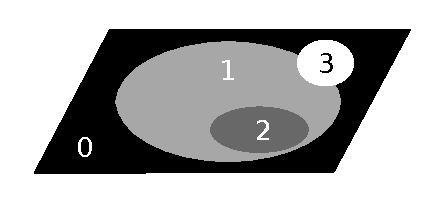
\includegraphics[trim= 0mm 0mm 0mm 5mm, clip, scale=0.75]{Formulation/figure/abc_img.pdf}}		    \hspace{0cm}
		    %\subfloat[$G_T=(S,A_T)$\label{fig:abc_graph_topo}]{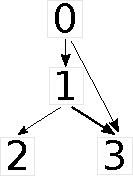
\includegraphics[scale=0.8]{Formulation/figure/abc_graph_topo.pdf}}	
		    \subfloat[Graphe $G_T$\label{fig:abc_graph_topo}]{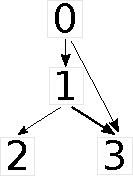
\includegraphics[trim= -10mm 0mm -10mm 0mm, clip, scale=0.8]{Formulation/figure/abc_graph_topo.pdf}}	\hspace{0cm}
		    %\subfloat[$G_P=(S,A_P)$\label{fig:abc_graph_photo}]{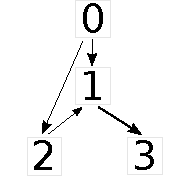
\includegraphics[scale=0.8]{Formulation/figure/abc_graph_photo.pdf}}	
		    \subfloat[Graphe $G_P$\label{fig:abc_graph_photo}]{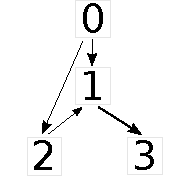
\includegraphics[trim= -10mm 0mm -10mm 0mm, clip, scale=0.8]{Formulation/figure/abc_graph_photo.pdf}}	\hspace{0cm}
		     \subfloat[Gradien $G_P$\label{fig:abc_graph_photo_gradient}]{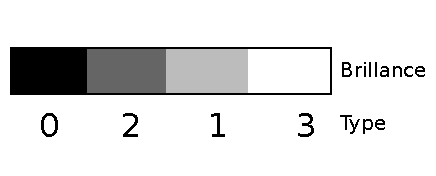
\includegraphics[trim= 0mm 0mm 0mm 0mm, clip, scale=0.5]{Formulation/figure/abc_graph_photo_gradient.pdf}}
		}\caption{ Exemple d'une image et des graphes conceptuels associés.}
         \label{fig:img_and_graph}
	\end{figure}
	%%%%%%%%%%%%%%%%%%%%%%%%%%%%%%%%%%%%%%%%%%%%%%%%%%%

	Selon l'image~\ref{fig:abc_img}, l'ensemble $S$ est égal à $\{0,1,2,3\}$. Sur le graphe~\ref{fig:abc_graph_topo} on représente les inclusions partielles et totales des régions. On voit que la région 2 est complètement incluse dans 1, qui est elle même incluse dans 0. La régions 3 quand à elle est incluse partiellement dans 1 et 2. Cette information se traduit par deux arcs entrant sur le n\oe{}ud 3 (fig.~\ref{fig:abc_graph_topo}). Dans le second graphe (fig.~\ref{fig:abc_graph_photo}), on représente les relations d'intensité lumineuse caractérisées par des arcs entrants (plus clair que) et sortant (plus sombre que). On retrouve par lecture du graphe, que 0 est la région la plus sombre (aucun arc entrant) et 3 la plus claire (aucun arc sortant). 
	
	La disposition spatiale des n\oe{}uds est identique pour les deux graphes pour souligner leurs différences limitées aux arcs qui les composent. Une autre représentation équivalente des informations photométriques peut être la figure~\ref{fig:abc_graph_photo_gradient} où l'on positionne les étiquettes des régions selon un gradient de niveaux de gris.

	%Note\footnote{la représentation en ligne de 1.1c) et plus simple à comprendre que celle sur la base de la structure topologique, mais cette dernière sera plus simple à implémenter si on combine les deux graphes. Que choisir? {\bf: cf propositions: la distribution spatiale des noeuds est la même dans les deux, permettant ainsi de souligner la différence entre info topo et photo.}}\\
	Par la suite, selon si les arcs traduisent une information topologique ou photométrique, nous aurons deux types de graphes, respectivement symbolisés par $G_T$ (fig.~\ref{fig:abc_graph_topo}) et $G_P$ (fig.~\ref{fig:abc_graph_photo} ), reposant sur les mêmes n\oe{}uds mais se distinguant selon les arcs :
	\begin{itemize}
		\item
		Topologique: $G_T=(S, A_T)$ %(actuellement: $F=G$, sans écrire mathématiquement que $F$ est un graphe associé à un ensemble de sommets ($S$) et d'arêtes (pas de notation)). 
		\item
		Photométrique: $G_P=(S,A_P)$
	\end{itemize}

	 Où $S$ est l'ensemble des n\oe{}uds (types) et $A_x$ l'ensemble des arcs les reliant.
	 
	Nous nous appuierons sur le formalisme de \citep[Fasquel]{Fasquel2006} en changeant quelques notations de sorte à rester cohérent avec notre étude. En effet dans son travail, il n'y avait pas de distinction de type d'arc car seule l'information topologique était considérée. L'intégration de la photométrie nécessite donc d'affiner les notations. On remplace $F$ par $G_T$ (pour graphe topologique), on utilise les notions de ``prédécesseurs/successeurs'' au lieu de ``pères/fils'' et on change l'orientation des arcs du graphe topologique. %pour être cohérent avec la \textbf{théorie des graphes [REF]}.


\subsection{Relations: illustration dans le cas topologique}

	Pour tous les éléments $i$ contenu dans l'ensemble $S$, $G_T^{+1}(i)$ est un sous ensemble de $S$ qui contient les ``successeurs''  directs (à une distance de +1) de $i$, $G_T^{-1}(i)$ ses prédécesseurs directs. Notons $G_T^{-1}(0) = \emptyset$ et $\forall i \in S,\; G_T(i) \subseteq S$. Une autre notation $G_{T}^{-\infty}(i)$, représente tous les ``prédécesseurs'' (jusqu'à la racine du graphe) d'un type $i$, par exemple, sur la figure~\ref{fig:a_priori_info},  $G_{T}^{-\infty}(4)=\{2,0\}$.


	%%%%%%%%%%%%%%%%%%%%%%%%%%%%%%%%%%%%%%%%%%%%%%%%%%%
	\begin{figure}[!ht]	%trim=l b r t
	  \centering
	      \fbox{
		  \subfloat[Graphe $(G_T)$]{\label{fig:a_priori_topo_graph}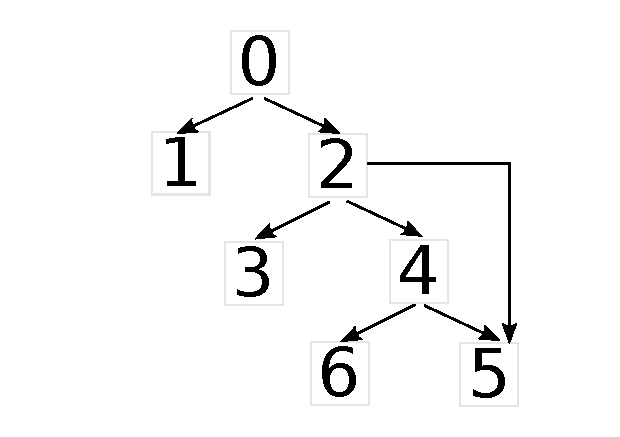
\includegraphics[trim= 0mm 5mm 0mm 5mm, clip, scale=0.3]{Formulation/figure/info_topo_graph.pdf}}
		  \subfloat[Image à priori $(I)$]{\label{fig:a_priori_topo_img}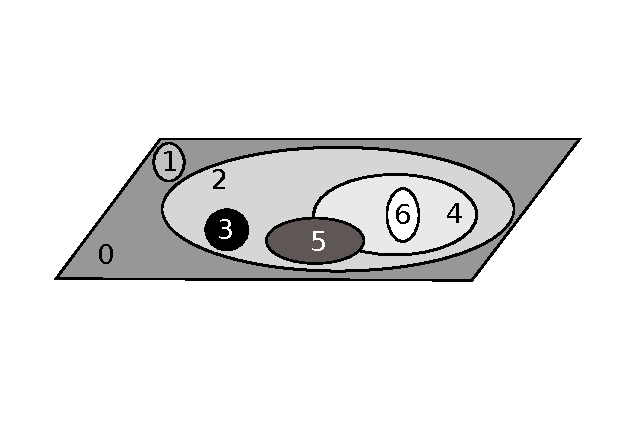
\includegraphics[trim= 0mm 20mm 0mm 15mm, clip, scale=0.4]{Formulation/figure/a_priori_img.pdf}}

		  %\fbox{\includegraphics[trim= 0mm 30mm 0mm 15mm, clip, scale=0.3]{Formulation/figure/info_topo.pdf}}	%trim=l b r t  width=0.5\textwidth, 

		  %\includegraphics[width=0.5\textwidth]{Formulation/figure/info_topo.pdf}
		}\caption{Exemple de représentation d'informations topologiques à priori.}
         \label{fig:a_priori_info}
	\end{figure}
	%%%%%%%%%%%%%%%%%%%%%%%%%%%%%%%%%%%%%%%%%%%%%%%%%%%

	Le graphe~\ref{fig:a_priori_topo_graph} représente un ensemble $S$ = \{0, 1, 2, 3, 4, 5, 6\} ayant des relations topologiques particulières définies par les arcs $A_T$, associées à une notion de recouvrement total ou partiel. On peut aisément déterminer les régions contenues (même partiellement) dans une région donnée en utilisant la notion de ``prédécesseurs'' : $G_T^{-1}(0)=\emptyset$, $G_T^{-1}(1) = \{0\}$, $G_T^{-1}(2) = \{0\}$, $G_T^{-1}(3) = \{2\}$, $G_T^{-1}(4) = \{2\}$, $G_T^{-1}(5) = \{2,4\}$, $G_T^{-1}(6) = \{4\}$. 

	Ou inversement, en utilisant la notion de ``successeurs'' : $G_T^{1}(0)=\{1,2\}$, $G_T^{1}(1) = \emptyset$, $G_T^{1}(2)=\{3,4,5\}$, $G_T^{1}(3)=\emptyset$, $G_T^{1}(4)=\{5,6\}$, $G_T^{1}(5)=\emptyset$, $G_T^{1}(6)=\emptyset$.

	Les informations à priori dépendent donc d'un ensemble de types $(S)$ qui ont des propriétés d'inclusion (arcs $A_T$ dans $G_T$), et de l'image $(I)$. On les note $C=\{G_T, I\}$.\vspace{1em}

	En considérant l'imagerie médicale comme domaine d'application, on peut associer les éléments de $S$ à des structures anatomiques (e.g. foie, rate) ou pathologiques (e.g. tumeur hépatique), ou bien à des structures relatives au système d'imagerie (e.g. table sur laquelle le patient est placé lors de l'acquisition de l'image). Ainsi, on pourrait par exemple assimiler ces régions à l'acquisition (0), la table sur laquelle est placée le patient dans l'imageur (1), le corps (2), la rate (3), le foie (4), un vaisseau hépatique (5) et une tumeur du foie (6). $G_T^{-1}(5)=\{4,2\}$ signifierait donc que le vaisseau hépatique est contenu par la région du foie et du corps mais pas par celle de la rate par exemple. 


      %{\bf Attention notation: $\mathbf{S}=\{0, ..., N\}$ puis (après) $S$ = \{A,B,C,D,E,F,G\}: rester homogène et ne considérer qu'une seule notation: soit 0..N, soit A..X : alternative privilégier 0...N (plus simple de manipuler des numéros que des lettres). On pourra éventuellement utiliser $S=\{L_0, ..., L_N\}$, ou $S=\{L_i \}$ avec $i=\{0,...,N\}$ L: étiquette associée à une région (Label en anglais).}

    \section{Intégration du processus d'analyse séquentiel}
	Dans le cadre d'un processus d'analyse séquentiel, il s'agit d'intégrer l'information relative aux régions déjà segmentées : les étapes de segmentation suivantes prennent alors en compte le contexte, à savoir les informations (contextuelles) sur les régions déjà identifiées \citep[Fasquel]{Fasquel2006}. Les informations contextuelles se distinguent des précédentes par un indice de temps qui s'apparente aux itérations. On les notera $C_t=\{G_{T,t}, I_t\}$ avec $G_{T,t}=(S_t,A_T)$.\\
	$G_{T,t}$ est équivalent à $G_T$ dans lequel seulement certains n\oe{}uds $u\in S_t$ sont valides (correspondant à des régions déjà segmentées, même partiellement). Pour pouvoir différencier visuellement, nous intégrerons la notion d'activation de noeud du graphe conceptuel initial, comme considéré récemment par \citep[Fasquel]{Fasquel2006} (voir fig.~\ref{fig:info_topo_context_graph}). Dans le même esprit, nous encadrerons en noir le type recherché. L'ensemble $S_t \subseteq S$ comprends tous les types de régions qui ont été segmentés jusqu'à $t-1$. A $t=0$, lors de la première séquence, on a $S_0=\{0\}$ car toute l'image est implicitement identifiée. Les arêtes de $G_{T,t}$ demeurent inchangées et correspondent à $A_T$.\\
	$\forall u \in S$, $G_{T,t}^{-1}(u)$ renvoie les prédécesseurs valides à $t$. Par exemple, dans la figure~\ref{fig:info_topo_context_graph}, où seul 1 et 4 ne sont pas valides, les prédécesseurs valides de 5 à $t$ sont définit par $G_{T,t}^{-1}(5)=\{2\}$.\\
	Tout comme $I$, $I_t = \{X_t(u)\;|\;u \in S_t\}$ (fig.~\ref{fig:topo_img}), où $X_t(u)$ est la région d'une structure $u$ déjà segmentée ($u \in S_t \Leftrightarrow X_t(u) \neq \emptyset$).


	%%%%%%%%%%%%%%%%%%%%%%%%%%%%%%%%%%%%%%%%%%%%%%%%%%%
	\begin{figure}[!ht]	%trim=l b r t  width=0.5\textwidth, 
	  \centering
	      \fbox{
		  \subfloat[Graphe ($G_{T,t}$)]{\label{fig:info_topo_context_graph}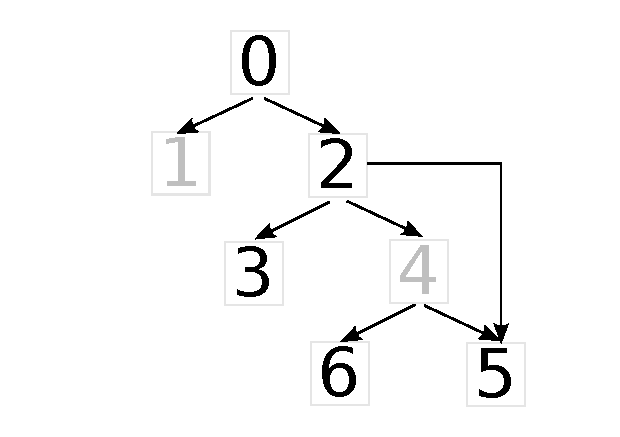
\includegraphics[trim= 0mm 5mm 0mm 0mm, clip, scale=0.3]{Formulation/figure/info_topo_context_graph.pdf}}
		  \subfloat[Image($I_t$)]{\label{fig:topo_img}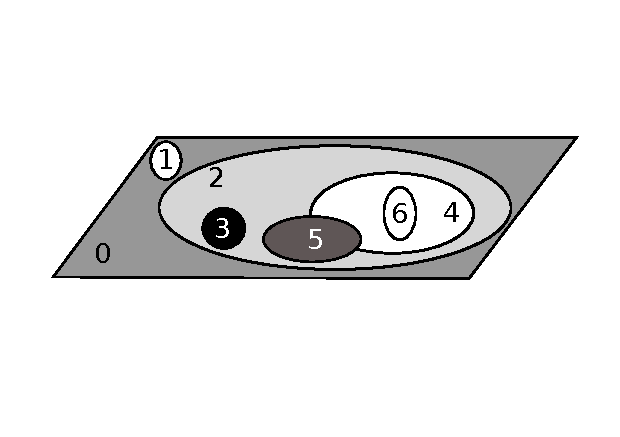
\includegraphics[trim= 0mm 15mm 0mm 10mm, clip, scale=0.47]{Formulation/figure/info_topo_context_image.pdf}}
		  \subfloat[Région de $R_t(5)$]{\label{fig:info_topo_context_image_ex}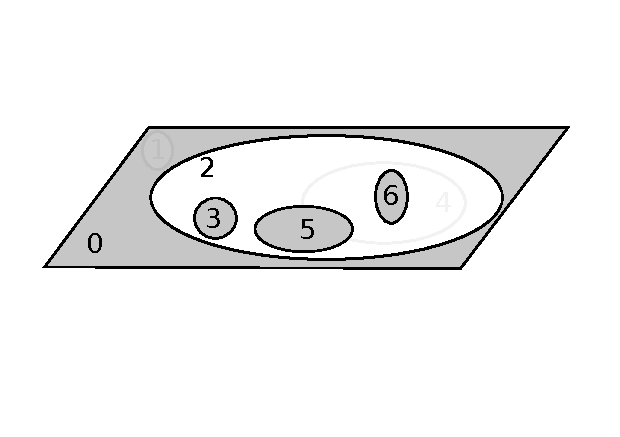
\includegraphics[trim= 0mm 18mm 0mm 10mm, clip, scale=0.5]{Formulation/figure/info_topo_context_image_ex.pdf}}
	      }\caption{Exemple d'information contextuelles à $t$. Les n\oe{}uds en gris sont dit invalidés, à l'inverse de ceux en noir qui sont valides. En faisant l'analogie avec la figure~\ref{fig:a_priori_info}, la table (1) et le foie (4) ne sont pas segmentés à cette date $t$. }
         \label{fig:contextual_info}
	\end{figure}
	%%%%%%%%%%%%%%%%%%%%%%%%%%%%%%%%%%%%%%%%%%%%%%%%%%%

\newpage
     \section{Inférence et topologie: région d'intérêt}

	On propose de reprendre la définition de la région d'intérêt (Region Of Interest) proposée par \citep[Fasquel]{Fasquel2006} qui défini la ROI optimale d'un type $u \in S$ comme :

	%%%%%%%%%%%%%%%%%%%%%%%%%%%%%%%%%%%%%%%%%%%%%%%%%%%
	\begin{equation}
		R_t(u)=\left(\bigcup_{l\in G_{T,t}^{-1}(u)}X_t(\overline{l})\right) \cup \left(\bigcup_{i\in S_t| u\in G_{T,t}^{-\infty}(i)}X_t(i) \right)
		\label{eq:roi}
	\end{equation}
	%%%%%%%%%%%%%%%%%%%%%%%%%%%%%%%%%%%%%%%%%%%%%%%%%%%

% 	\begin{center}
% 		\begin{tabular}{ll}
% 		$t$ 		& : numéro (date) d'une itération \\
% 		$u$ 		& : type recherché (cible) \\
% 		$i$		& : type générique appartenant à l'ensemble $S$ \\
% 		$l$ 		& : élément (liaison) du sous ensemble $F_t$ \textbf{???}\\
% 		            & {\bf élément de l'ensemble des prédécesseurs (dans $S_t$)}:\\
% 				 & {\bf étiquette d'une des régions déjà segmentées contenant (au moins partiellement) $u$}\\
% 		$\bar{l}$	& : \textbf{???} \\
% 		$R_t(u)$ 	& : ROI optimale au sens [Fasquel] d'un type $u$ \\
% 		$F_t(u)$ 	& : les informations inter-régions (inter-n\oe{}uds) à $t$ qui concernent la cible $u$ \\
% 		$X_t(\bar{l})$ 	& : région d'une structure $\bar{l}$ déjà segmentée \textbf{???} {\bf (voir ci-dessous)}\\
% 		$X_t(i)$ 	& : région d'une structure $i$ déjà segmentée \\
%  		$F^\infty(i)$ 	& : ensemble des ancêtres de l'élément $i$ (jusqu'au ``root'') \\
% 		$S_t$ 		& : ensemble des types de régions qui ont étaient segmentés entre $t$ et $t-1$ \\
% 		\end{tabular}
% 	\end{center}	 
% 
% {\bf $\bar{l}$: résidu vs l (voir article pour définition). En terme d'images, cela correspond à ce qui reste d'une région quand on a enlevé toutes les régions (dont les étiquettes sont les prédécesseurs de $l$ dans le graphe) qu'elle peut contenir: ce reste est une région dont le labele/étiquette/identité est $\bar{l}$. Cette étiquette correspond à un noeud implicite du graphe.}

	Le premier membre correspond à l'union des prédécesseurs directs de la cible. La région est réduite autour de la cible par les informations contextuelles des relations, symbolisées par $G_{T,t}$. En fait, cette réduction est réalisée par suppression des régions déjà segmentées qui intersectent les régions supposées contenir la cible (au moins partiellement). Ces structures peuvent être du même type que la cible recherchée mais on suppose que deux structures du même type ne s'intersectent pas.

	Le second terme vérifie que les régions qui recouvrent partiellement la cible soit conservées dans la ROI. Cela permet par exemple de ne pas supprimer une partie du foie qui serai recouverte par le vaisseau hépatique en supprimant le vaisseau hépatique.

	Prenons par exemple, une cible de type $6$ (tumeur du foie) :

	%%%%%%%%%%%%%%%%%%%%%%%%%%%%%%%%%%%%%%%%%%%%%%%%%%%
	\begin{equation}
		R_t(6)=\left(\bigcup_{l\in G_{T,t}^{-1}(6)}X_t(\overline{l})\right) \cup \left(\bigcup_{i\in S_t| 6\in G_{T,t}^{-\infty}(i)}X_t(i) \right)
		\label{eq:roi_ex}
	\end{equation}
	%%%%%%%%%%%%%%%%%%%%%%%%%%%%%%%%%%%%%%%%%%%%%%%%%%%

	De part les informations contextuelles rappelées sur la figure~\ref{fig:info_topo_context_graph}, on a $\{l \in G_{T,t}^{-1}(6)\} = G_{T,t}^{-1}(6) = \{2\}$ et $\{i \in S_t \;|\;6\in G_{T,t}^{-\infty}(i) \}=\emptyset$ ce qui nous amène à $R_t(6)=X_t(2) \setminus (X_t(3) \cup X_t(5) \cup X_t(6))$ . On  représente cette région en blanc sur la figure~\ref{fig:info_topo_context_image_ex}.


	%%%%%%%%%%%%%%%%%%%%%%%%%%%%%%%%%%%%%%%%%%%%%%%%%%%
% 	\begin{figure}[!ht]	% ! here top bottom
% 	  \centering
% 	      \fbox{
% 		  \subfloat[Graphe ($G_{T,t}$)]
% 		  {\label{fig:info_topo_context_graph_ex}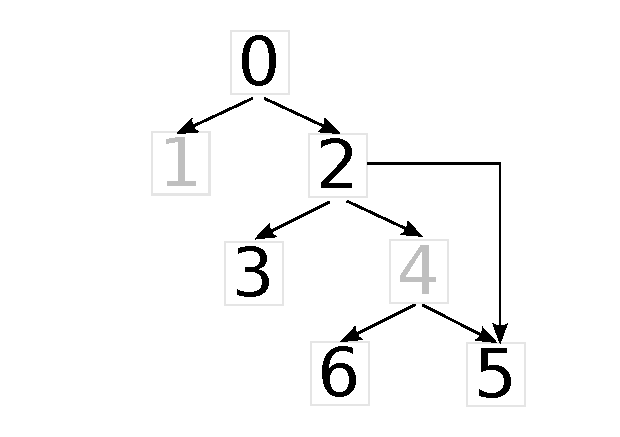
\includegraphics[trim= 0mm 5mm 0mm 5mm, clip, scale=0.3]{Formulation/figure/info_topo_context_graph_ex.pdf}}	%trim=l b r t
% 		  \subfloat[Région de $R_t(6)$]{\label{fig:info_topo_context_image_ex}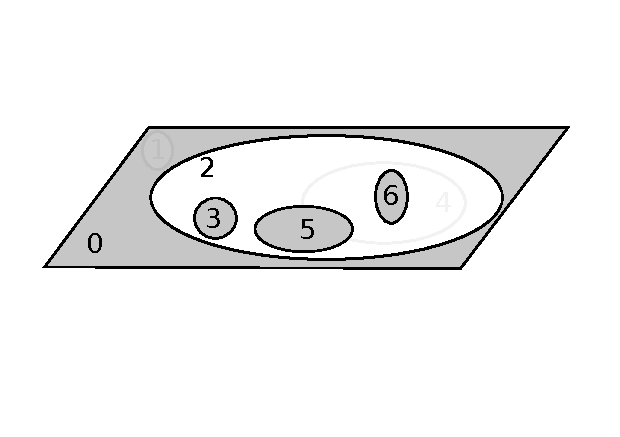
\includegraphics[trim= 0mm 20mm 0mm 15mm, clip, scale=0.5]{Formulation/figure/info_topo_context_image_ex.pdf}}	%trim=l b r t  width=0.5\textwidth, 
% 	      }\caption{Graphe d'informations contextuelles. {\bf tu devrais faire une seule figure avec \ref{fig:contextual_info}: sous-figure (b) de \ref{fig:contextual_info_rappel_ex} devient (c) dans fig. \ref{fig:contextual_info}}}
%          \label{fig:contextual_info_rappel_ex}
% 	\end{figure}
	%%%%%%%%%%%%%%%%%%%%%%%%%%%%%%%%%%%%%%%%%%%%%%%%%%%


% \newpage
%       \subsubsection{Nombre de classes}
% 
% 	Nous définissons le nombre de classes par la cardinalité de l'ensemble des n\oe{}uds non segmentés (ensemble des n\oe{}uds moins les n\oe{}uds déjà segmentés) appartenant à la ROI. Ici nous considérons toutes les classes possibles en omettant l'aspect optionnel des types pathologiques. Ce nombre est définit par la formule suivante :
% 
% 	%%%%%%%%%%%%%%%%%%%%%%%%%%%%%%%%%%%%%%%%%%%%%%%%%%%
% 	\begin{equation}
% 		%N_t(u) = \operatorname{Card}\{X_t(i) \in R_t(u) \; \forall \;i\}
% 		N_t(u) = \operatorname{Card}\{i \in S \setminus S_t \;|\; X(i) \in R_t(u)\}
% 		%nbClMax = \operatorname{Card}\{R_t(u)\}
% 		\label{eq:nb_classe}
% 	\end{equation}
% 	%%%%%%%%%%%%%%%%%%%%%%%%%%%%%%%%%%%%%%%%%%%%%%%%%%%
% 
% 	\begin{center}
% 		\begin{tabular}{ll}
% 		$u$ 	& : n\oe{}ud correspondant à un type de structure (cible) \\
% 		$i$	& : élément (intersection) de l'ensemble $S$ \\
% 		$N_t(u)$& : nombre de classes attendue pour le n\oe{}ud $u$ \\
% 		$R_t(u)$& : ROI en fonction d'une structure cible $u$ \\
% 		$X(i)$	& : région d'une structure cible $i$ issue de l'ensemble de structures $S$ au temps $t$\\
% 		$S_t$ 	& : ensemble des types de régions qui ont étaient segmentés entre $t$ et $t-1$ \\
% 		$S$ 	& : ensemble des structures à priori \\
% 		\end{tabular}
% 	\end{center}
% 
% 	%%%%%%%%%%%%%%%%%%%%%%%%%%%%%%%%%%%%%%%%%%%%%%%%%%%
% 	\begin{figure}[!ht]
% 	  \centering
% 	      \subfloat[Graphe]{\label{fig:info_topo_nb_class}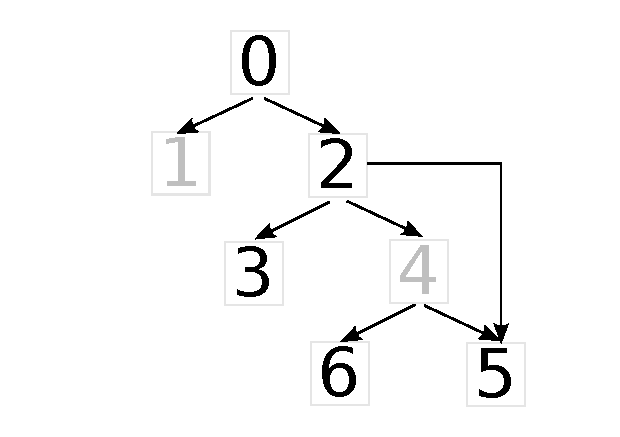
\includegraphics[trim= 0mm 5mm 0mm 5mm, clip, scale=0.3]{Formulation/figure/info_topo_context_graph.pdf}}	%trim=l b r t  width=0.5\textwidth, 
% 		\subfloat[Image]{\label{fig:topo_img}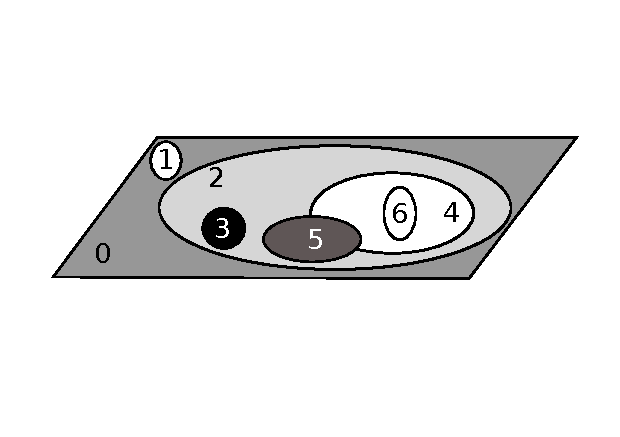
\includegraphics[trim= 0mm 30mm 0mm 15mm, clip, scale=0.4]{Formulation/figure/info_topo_context_image.pdf}}	%trim=l b r t 
% 	      \caption{Exemple de recherche du nombre de classes. }
%          \label{fig:contextual_info}
% 	\end{figure}
% 	%%%%%%%%%%%%%%%%%%%%%%%%%%%%%%%%%%%%%%%%%%%%%%%%%%%
%\newpage
    \section{Inférence et photométrie}
    \label{sec:inf_and_photo}
	Les déductions faites à partir des connaissances disponibles à $t$ par le moteur d'inférence\footnote{Moteur d'inférence : de l'anglais ``enference engine'' et du verbe ``inférer'' qui signifie ``déduire'', c'est un concept de raisonnement déductif à qui on demande des informations et qui déduit des conclusions à partir d'une base de faits et d'une base de connaissances.}, portent sur les propriétés photométriques de la région au sein de laquelle vont s'effectuer les traitements. 

Ces propriétés photométriques que l'on propose d'inférer, concernent le nombre de classes ``photométriques'' de la ROI ainsi que leurs relations d'ordres, permettant ainsi d'associer une classe à un noeud du graphe, c'est à dire à une région bien identifiée. Il est à noter que ces déductions dépendent de celles considérées dans la section précédente au sujet de la région d'intérêt optimale.

Pour cette première phase de l'étude, nous faisons l'hypothèse simplificatrice que toutes les régions ont une multiplicité de 1. Cela signifie qu'elles sont dans l'image (aucune n'est optionnelle) et qu'elles sont uniques, il ne peut donc pas y avoir deux tumeurs hépatiques par exemple.

      \subsection{Nombre de classes}
	%Ici nous considérons tous les types possibles en omettant l'aspect optionnel ou multiple des types pathologiques. Une multiplicité de un, signifie que chaque type est unique dans l'image, il ne peut donc pas y avoir deux tumeurs hépatiques par exemple. 
	L'objectif est d'isoler un sous-ensemble à priori de types correspondant aux lobes issues d'une région d'intérêt dans l'histogramme d'une image. On présente ci-dessous les étapes majeures qui ont contribué à l'établissement de la formule finale.

	Dans un premier temps, nous utilisons la notion de ``ROI optimale'' présentée dans la section précédente pour déterminer un sous-ensemble nommé $L_t(u)$. Ce sous-ensemble est composé de l'ensemble des types non segmentés ($S \setminus S_t$) inclus dans la région d'intérêt d'un type $u$ et de ses prédécesseurs directs ($G_{T,t}^{-1}(u)$). Formule initiale :

	%%%%%%%%%%%%%%%%%%%%%%%%%%%%%%%%%%%%%%%%%%%%%%%%
	\begin{equation}
		%N_t(u) = \operatorname{Card}\{X_t(i) \in R_t(u) \; \forall \;i\}
		L_t(u) = \{i \in S \setminus S_t \;|\; X(i) \in R_t(u)\} \cup G_{T,t}^{-1}(u)
		%L_t(u) = \{i \in S \setminus S_t \;|\; X(i) \in R_t(u) \; AND \; G_{P,t}^{[u,iMin]} \}
		%nbClMax = \operatorname{Card}\{R_t(u)\}
		\label{eq:nb_lobe}
	\end{equation}
	%%%%%%%%%%%%%%%%%%%%%%%%%%%%%%%%%%%%%%%%%%%%%%%%

	Durant l'expérimentation de cette formule, nous nous sommes demandé si l'on pouvait la simplifier du fait que la région $R_t(u)$ et les successeurs $G_{T,t}^{-1}(u)$ utilisaient les mêmes informations à priori. En effet la région peut être exprimée par l'ensemble des successeurs des prédécesseurs de $u$ : $G_T^{\infty}(G_{T,t}^{-1}(u))$.	La formule précédente devient :

	%%%%%%%%%%%%%%%%%%%%%%%%%%%%%%%%%%%%%%%%%%%%%%%%
	\begin{equation}
	L_t(u) =  \{ i\in S \setminus S_t|\; i \in G_T^{\infty}(G_{T,t}^{-1}(u))\} \cup G_{T,t}^{-1}(u)
	\end{equation}
	%%%%%%%%%%%%%%%%%%%%%%%%%%%%%%%%%%%%%%%%%%%%%%%%

	Elle peut se simplifier en remplaçant le premier membre par l'intersection de l'ensemble non segmenté avec l'ensemble des successeurs des prédécesseurs : 

%remplaçant l'union de l'ensemble de ses successeurs non segmentés d'un type de $\{ i\in S \setminus S_t|\; i \in G_T^{\infty}(i)\}$ par $G_T^{\infty}(k) \cap \{S \setminus S_t\}$. :

	%%%%%%%%%%%%%%%%%%%%%%%%%%%%%%%%%%%%%%%%%%%%%%%%
	\begin{equation}
		L_t(u) = \left\{ ( S \setminus S_t ) \cap  G_T^{\infty}(G_{T,t}^{-1}(u)) \right\} \cup G_{T,t}^{-1}(u)
	\end{equation}
	%%%%%%%%%%%%%%%%%%%%%%%%%%%%%%%%%%%%%%%%%%%%%%%%

	Une forme plus généraliste de $L_t(u)$ pourrait être, pour un élément $i$ issu des prédécesseurs de $u$ ($i\in G_{T,t}^{-1}(u)$), l'union de l'ensemble des successeurs non segmentés dont les prédécesseurs actifs font parti de $G_{T,t}^{-1}(u)$ et des prédécesseurs de $u$ eux-mêmes ($G_{T,t}^{-1}(u)$). 

	%%%%%%%%%%%%%%%%%%%%%%%%%%%%%%%%%%%%%%%%%%%%%%%%
	\begin{equation}
		L_t(u) =  \left(\bigcup_{i\in G_{T,t}^{-1}(u)} ( S \setminus S_t ) \cap G_T^{\infty}(i) \right) \cup G_{T,t}^{-1}(u) 
	\end{equation}
	%%%%%%%%%%%%%%%%%%%%%%%%%%%%%%%%%%%%%%%%%%%%%%%%

	Nous avons pu constater lors de tests, une faiblesse de cette formule dans des cas limites comme lorsque l'origine du graphe (0) fait parti des prédécesseurs de $u$ ou encore quand $u$ a plusieurs prédécesseurs actifs.% lorsque la racine du graphe $G_t(0)$ faisait partie de l'ensemble $G_{T,t}^{-1}(u)$. Dans ce cas, $G_T^{\infty}(G_{T,t}^{-1}(u))$ est égal à l'ensemble des n\oe{}uds de $S$ ce qui fausse le résultat puisque qu'il contient des types non actif successeurs de types actifs. Nous devons donc les soustraire : $G_T^{\infty}(G_{T,t}^{-1}(u)) \setminus G_T^{\infty} (G_{T,t}^{+1}(G_{T,t}^{-1}(u)) )$. Dans la formule suivante on notera l'ensemble des successeurs valides $G_{T,t}^{-1}(u)=U$ pour alléger les notations.


	%%%%%%%%%%%%%%%%%%%%%%%%%%%%%%%%%%%%%%%%%%%%%%%%
% 	\begin{equation}
% 	      L_t(u) = \left\{ ( S \setminus S_t ) \cap ( G_T^{\infty}(U) \setminus G_T^{\infty} (G_{T,t}^{+1}(U) ) ) \right\} \cup U 
% 	\end{equation}
	%%%%%%%%%%%%%%%%%%%%%%%%%%%%%%%%%%%%%%%%%%%%%%%%
	
% 	Simplification proposée :
% 
% 	%%%%%%%%%%%%%%%%%%%%%%%%%%%%%%%%%%%%%%%%%%%%%%%%%%%
% 	\begin{equation}
% 	  %L_t(5) = & \left( ( S \setminus S_t ) \cap G_{T}^\infty \left( G_T^{-1}(5) \setminus G_{T,t}^{-1} \left( 5 \right) \right) \right) \cup G_{T,t}^{-1}(5) \\
% 	 L_t(u) = \left( ( S \setminus S_t ) \cap \left( G_T^{+1}(i) \;|\; i \in G_{T,t}^{-1}(u) \right) \right) \cup G_{T,t}^{-1}(u)
% 	\end{equation}
	%%%%%%%%%%%%%%%%%%%%%%%%%%%%%%%%%%%%%%%%%%%%%%%%%%%

	Nous proposons donc la formule suivante qui renvoie l'ensemble des types qui succèdent aux prédécesseurs de $u$ ($G_T^{\infty}(G_{T,t}^{-1} (u))$), non actifs, ($\cap\; S \setminus S_t$), et qui ont au moins un prédécesseur actif direct en commun avec $u$ ($G_{T,t}^{-1} (i) \cap G_{T,t}^{-1} (u) \neq \emptyset$). A cet ensemble on ajoute l'ensemble des prédécesseurs de $u$ avec $G_{T,t}^{-1}(u)$ :
	%%%%%%%%%%%%%%%%%%%%%%%%%%%%%%%%%%%%%%%%%%%%%%%%%%%
	\begin{equation}
 	  L_t(u) = \left\{ i \in \left( G_T^{\infty}(G_{T,t}^{-1} (u)) \cap ( S \setminus S_t ) \right) \;|\; \left( G_{T,t}^{-1} (i) \cap G_{T,t}^{-1} (u) \neq \emptyset \right) \right\} \cup  G_{T,t}^{-1}(u)\\
	\end{equation}
	%%%%%%%%%%%%%%%%%%%%%%%%%%%%%%%%%%%%%%%%%%%%%%%%%%%


	De cette relation, nous pouvons à présent compter le nombre de lobes $N_t$ attendus dans l'image à $t$ par la cardinalité (nombre d'éléments) du sous-ensemble $L_t(u)$ : $ N_t(u) = \left|{L_t(u)}\right|$. Rappelons que le nombre de lobes à priori est calculé pour optimiser le paramétrage d'algorithmes de segmentation.
	
		\subsubsection*{Exemples applicatifs}
	Application à une image, qui a les propriétés topologiques $G_{T,t}$, dans laquelle on cherche toutes les lobes à priori pour une ROI dans le but de les dénombrer puis de les identifier. On fera un aperçu du résultat graphique sur l'histogramme représentatif d'une image, dans lequel nous ferons apparaître les lobes correspondant aux types segmentés en trait plein. Les lobes en trait discontinu sont considérées comme inconnues. La position des lobes dans l'histogramme et leurs niveaux de gris (en abscisse de l'histogramme) sont représentés selon les informations photométriques à priori issue du graphe $G_P$ associé. Ce dernier ne sera utilisé qu'à titre d'illustration dans cette section (aucune utilisation de son information).\vspace{1em}

\begin{itemize}
\item Cas 1 : recherche du type $1$ sachant que les types $0$ et $2$ ont été segmentés :
\end{itemize}

	%%%%%%%%%%%%%%%%%%%%%%%%%%%%%%%%%%%%%%%%%%%%%%%%%%%
	\begin{figure}[!ht]	%trim=l b r t  width=0.5\textwidth,
	  \centering
	      \fbox{
		  \subfloat[Graphe $G_{T,t}$]{\label{fig:cas_1_graph_topo}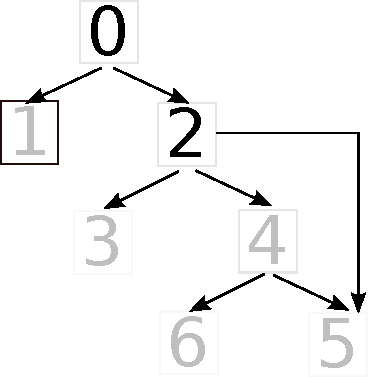
\includegraphics[trim= -10mm 0mm -10mm 0mm, clip, scale=0.4]{Formulation/figure/cas_1_graph_topo.pdf}}
		  %\subfloat[Région $R_t(1)$]{\label{fig:cas_1_img}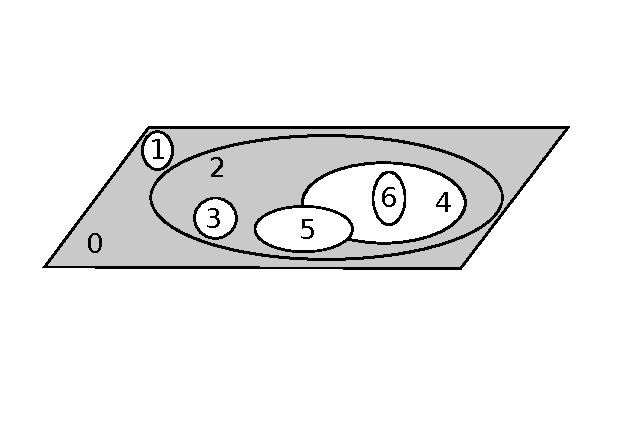
\includegraphics[trim= 8mm 5mm 10mm 5mm, clip, scale=0.5]{Formulation/figure/cas_1_img.pdf}}
		  \subfloat[Histogramme]{\label{fig:cas_1_histo}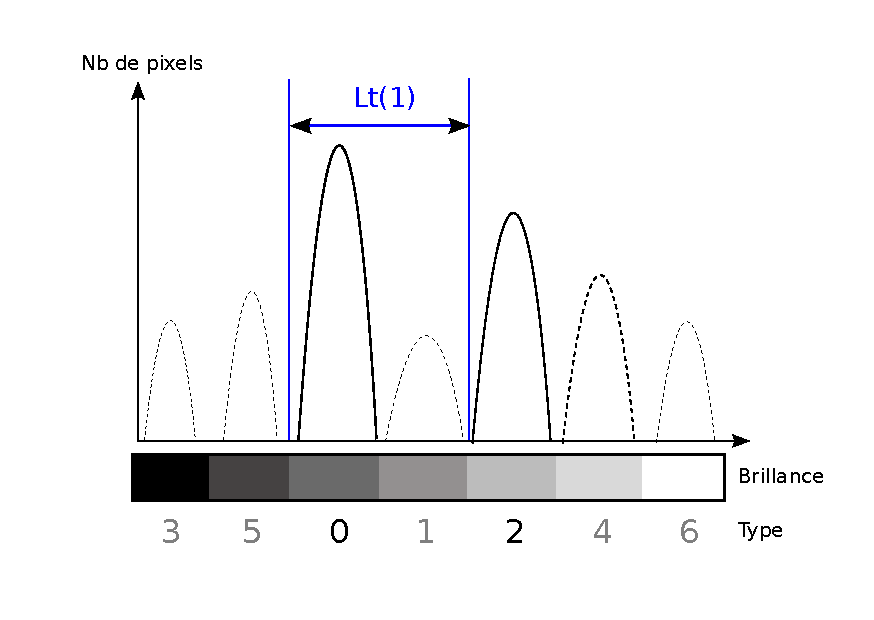
\includegraphics[trim= 0mm 10mm 0mm 5mm, clip, scale=0.4]{Formulation/figure/cas_1_histo.pdf}}
		  \subfloat[Graphe $G_{P,t}$]{\label{fig:cas_1_graph_photo}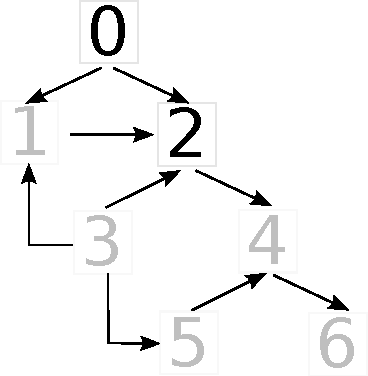
\includegraphics[trim= -10mm -5mm -10mm 0mm, clip, scale=0.4]{Formulation/figure/cas_1_graph_photo.pdf}}
	      }\caption{Sous-ensemble $L_t(1)$.}
	  \label{fig:cas_1}
	\end{figure}
	%%%%%%%%%%%%%%%%%%%%%%%%%%%%%%%%%%%%%%%%%%%%%%%%%%%


	%%%%%%%%%%%%%%%%%%%%%%%%%%%%%%%%%%%%%%%%%%%%%%%%%%%
	\begin{equation}
	 \begin{split}
	  L_t(1) = & \left\{ i \in \left( G_T^{\infty}(G_{T,t}^{-1}(1)) \cap ( S \setminus S_t ) \right) \;|\; \left( G_{T,t}^{-1} (i) \cap G_{T,t}^{-1} (1) \neq \emptyset \right) \right\} \cup  G_{T,t}^{-1}(1)\\
		 = & \left\{ i \in \left( \{1,2,3,4,6,5\} \cap \{1,3,4,6,5\} \right) \;|\; \left( G_{T,t}^{-1} (i) \cap \{0\} \neq \emptyset \right) \right\} \cup  \{0\}\\
		 = & \left\{1 \right\} \cup  \{0\}\\
	 \end{split}
	 \label{eq:cas1}
	\end{equation}
	%%%%%%%%%%%%%%%%%%%%%%%%%%%%%%%%%%%%%%%%%%%%%%%%%%%

	Le type 2 étant segmenté, il est exclu du sous-ensemble ($S \setminus S_t$) ainsi que les types 3, 4, 5 et 6 car ils n'ont pas de prédécesseurs direct en commun avec ceux de 1 $\left( G_{T,t}^{-1} (i) \cap G_{T,t}^{-1} (u) \neq \emptyset \right)$. Selon le graphe topologique figure~\ref{fig:cas_1_graph_topo}. Le deuxième membre $G_{T,t}^{-1}(1) = \{0\}$ car 1 n'a que 0 comme prédécesseur valide, il en résulte un ensemble de types $L_t(1) =  \{1, 0\}$. Cet ensemble est représenté sur la figure~\ref{fig:cas_1_histo} selon $G_{P}$ (fig.~\ref{fig:cas_1_graph_photo}). Sa cardinalité $N_t(1)=\left|{L_t(1)}\right| = 2$.\vspace{1em}
	
\begin{itemize}
\item 	Cas 2 : recherche du type $3$ sachant que les types 0, 1 et 2 ont été segmentés :
\end{itemize}

	%%%%%%%%%%%%%%%%%%%%%%%%%%%%%%%%%%%%%%%%%%%%%%%%%%%
	\begin{figure}[!ht]	%trim=l b r t  
	  \centering
	      \fbox{		  
		  \subfloat[Graphe $G_{T,t}$]{\label{fig:cas_2_graph_topo}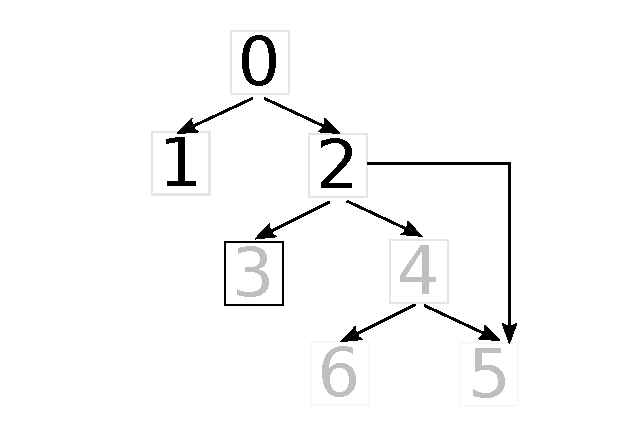
\includegraphics[trim= 20mm 0mm 0mm 5mm, clip, scale=0.4]{Formulation/figure/cas_2_graph_topo.pdf}}
		  \subfloat[Histogramme]{\label{fig:cas_2_histo}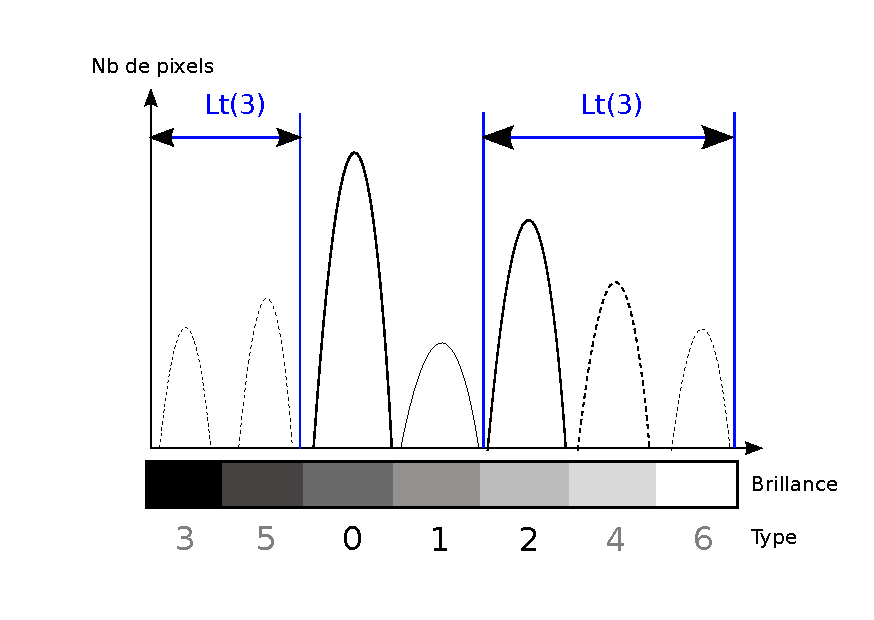
\includegraphics[trim= 0mm 10mm 0mm 5mm, clip, scale=0.4]{Formulation/figure/cas_2_histo.pdf}}
		  \subfloat[Graphe $G_{P,t}$]{\label{fig:cas_2_graph_photo}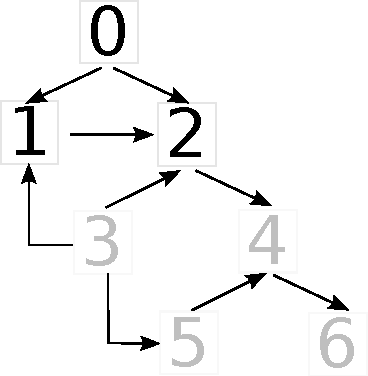
\includegraphics[trim= -10mm -5mm -10mm 0mm, clip, scale=0.4]{Formulation/figure/cas_2_graph_photo.pdf}}
	      }\caption{Sous-ensemble $L_t(3)$.}
         \label{fig:cas_2}
	\end{figure}
	%%%%%%%%%%%%%%%%%%%%%%%%%%%%%%%%%%%%%%%%%%%%%%%%%%%

	%%%%%%%%%%%%%%%%%%%%%%%%%%%%%%%%%%%%%%%%%%%%%%%%%%%
	\begin{equation}
	 \begin{split}
	  L_t(3) = & \left\{ i \in \left( G_T^{\infty}(G_{T,t}^{-1}(3)) \cap ( S \setminus S_t ) \right)\;|\; \left( G_{T,t}^{-1} (i) \cap G_{T,t}^{-1} (3) \neq \emptyset \right) \right\} \cup  G_{T,t}^{-1}(3)\\
		 = & \left\{ i \in \left( G_T^{\infty}(\{2\}) 		\cap \{3,4,6,5\} 	 \right)\;|\; \left( G_{T,t}^{-1} (i) \cap \{2\} \neq \emptyset \right) \right\} \cup \{2\} \\
		 = & \left\{ 3,4,6,5 \right\} \cup \left\{ 2 \right\} \\
	 \end{split}
	 \label{eq:cas2}
	\end{equation}
	%%%%%%%%%%%%%%%%%%%%%%%%%%%%%%%%%%%%%%%%%%%%%%%%%%%

	Ici l'ensemble des types non segmentés $S \setminus S_t = \{3,4,5,6\}$ sont conservés car ils ont tous le même prédécesseur (fig.~\ref{fig:cas_2_graph_topo}). Le deuxième membre $G_{T,t}^{-1}(3) = \{2\}$ (seul prédécesseur valide de 3), il en résulte un ensemble de types $L_t(3) = \{3,4,6,5,2\}$. Cet ensemble est représenté sur l'histogramme~\ref{fig:cas_2_histo}. Sa cardinalité $N_t(3) = \left|{L_t(3)}\right| = 5$.\vspace{1em}

  %En revanche, de part les relations photométriques (fig.~\ref{fig:cas_2_graph_photo}) seul les types 3 et 5 sont conservés puisque 4 et 6 sont plus brillants que les types segmentés (régions connues). Il en résulte un ensemble de lobes $L_t(3) =  \{5,3\}$. 
%{\bf A mon avis, si l'on cherche 3, la ROI est en effet restreinte à $X_t(2)$, et il y aura 5 lobes, sans même regarder la formule: $L_t(3) =  \{2,3,4,5,6\}$, $2$ correspondant au fond de la ROI. Si on applique la formule suivante: $L_t(u) = \{i \in S \setminus S_t \;|\; X(i) \in R_t(u)\} \cup \{ G_{T,t}^{-1}(u) \}$:

% \begin{itemize}
% \item
% $\{i \in S \setminus S_t \;|\; X(i) \in R_t(3)\} = \{3,4,5,6\}$
% \item
% $\{ G_{P,t}^{-1}(3) \} = \{2\}$
% \end{itemize}
% Il semblerait que l'on tombe sur le bon résultat. Même remarque que pour cas 1 pour la figure \ref{fig:cas_2}. Ne pas faire apparaître le graphe photométrique (seulement partie "identification des lobes").

%\newpage
\begin{itemize}
\item Cas 3 : recherche du type $4$ sachant que les types 0, 2, 3, 5 et 6 ont été segmentés :
\end{itemize}

	%%%%%%%%%%%%%%%%%%%%%%%%%%%%%%%%%%%%%%%%%%%%%%%%%%%
	\begin{figure}[!ht]	%trim=l b r t  width=0.5\textwidth,
	  \centering
	      \fbox{
		  \subfloat[Graphe $G_{T,t}$]{\label{fig:cas_3_graph_topo}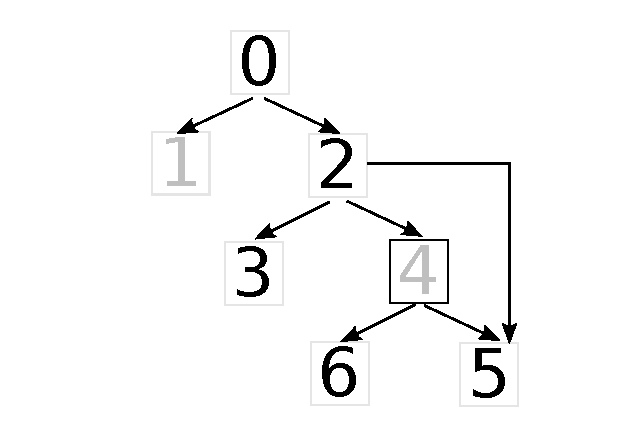
\includegraphics[trim= 20mm 5mm 0mm 5mm, clip, scale=0.4]{Formulation/figure/cas_3_graph_topo.pdf}}
		  %\subfloat[Image masquée]{\label{fig:cas_2_img}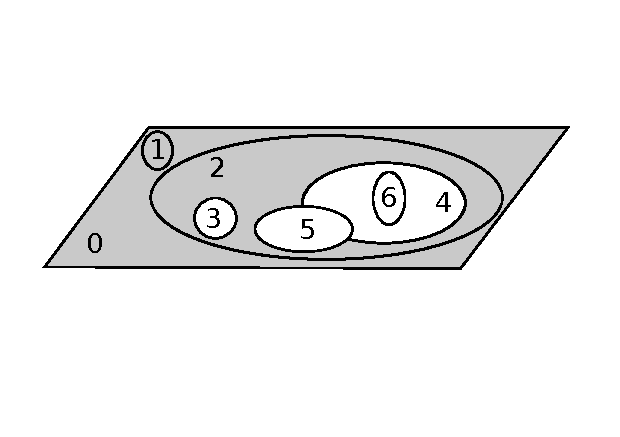
\includegraphics[trim= 8mm 20mm 10mm 5mm, clip, scale=0.5]{Formulation/figure/cas_2_img.pdf}}
		  \subfloat[Histogramme]{\label{fig:cas_3_histo}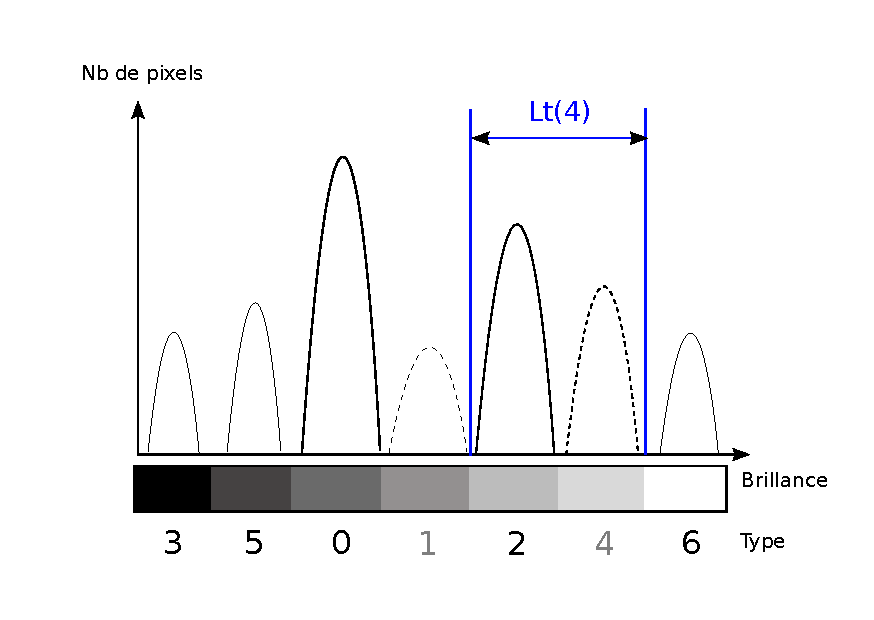
\includegraphics[trim= 0mm 10mm 0mm 5mm, clip, scale=0.4]{Formulation/figure/cas_3_histo.pdf}}
		  \subfloat[Graphe $G_{P,t}$]{\label{fig:cas_3_graph_photo}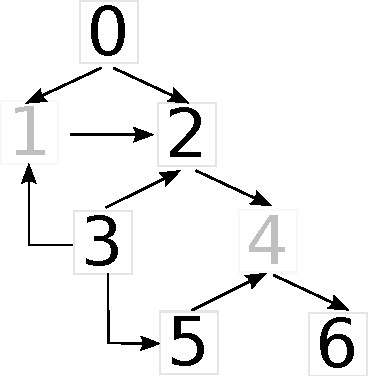
\includegraphics[trim= -10mm 0mm -10mm 0mm, clip, scale=0.4]{Formulation/figure/cas_3_graph_photo.pdf}}
	      }\caption{Sous-ensemble $L_t(4)$.}
         \label{fig:cas_3}
	\end{figure}
	%%%%%%%%%%%%%%%%%%%%%%%%%%%%%%%%%%%%%%%%%%%%%%%%%%%

	%%%%%%%%%%%%%%%%%%%%%%%%%%%%%%%%%%%%%%%%%%%%%%%%%%%
	\begin{equation}
	\begin{split}
	 L_t(4) = & \left\{ i \in \left( G_T^{\infty}(G_{T,t}^{-1}(4)) \cap ( S \setminus S_t ) \right)\;|\; \left( G_{T,t}^{-1} (i) \cap G_{T,t}^{-1} (4) \neq \emptyset \right) \right\} \cup  G_{T,t}^{-1}(4)\\
		= & \left\{ i \in \left( \{3,4,6,5\} \cap \{1,4\} \right)\;|\; \left( G_{T,t}^{-1} (i) \cap \{2\} \neq \emptyset \right) \right\} \cup  \{2\}\\
		= & \left\{ 4 \right\} \cup \left\{ 2 \right\} \\
	\end{split}
	\end{equation}
	%%%%%%%%%%%%%%%%%%%%%%%%%%%%%%%%%%%%%%%%%%%%%%%%%%%

	Parmi l'ensemble des types non segmentés $S \setminus S_t = \{1,4\}$, seul 4 a un prédécesseur identique à $u$ (fig.~\ref{fig:cas_3_graph_topo}). Le deuxième membre $G_{T,t}^{-1}(4) = \{2\}$ vient compléter l'ensemble $L_t(4) = \{4,2\}$. Cet ensemble est représenté sur l'histogramme~\ref{fig:cas_3_histo}. Sa cardinalité $N_t(4) = \left|{L_t(4)}\right| = 2$.\vspace{1em}
 
% 	%%%%%%%%%%%%%%%%%%%%%%%%%%%%%%%%%%%%%%%%%%%%%%%%%%%
% 	\begin{figure}[!ht]
% 	  \centering
% 	      \fbox{
% 		  %\subfloat[Graphe ($T_t$)]{\label{fig:info_topo_cas_1}\includegraphics[trim= 0mm 5mm 0mm 5mm, clip, scale=0.3]{Formulation/figure/info_topo_cas_1.pdf}}	%trim=l b r t  width=0.5\textwidth,
% 		  \subfloat[Image masquée]{\label{fig:image_ex}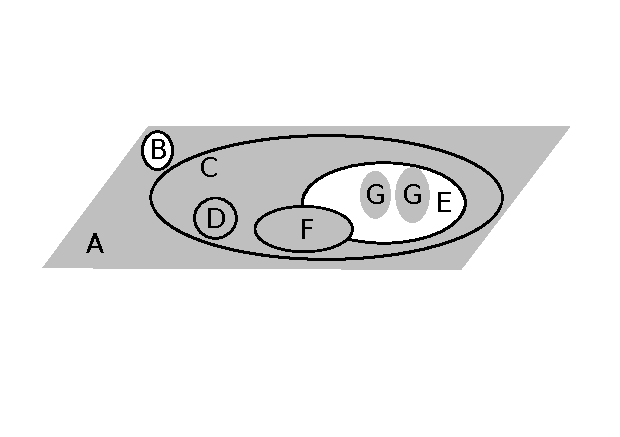
\includegraphics[trim= 0mm 20mm 0mm 5mm, clip, scale=0.5]{Formulation/figure/lobe_image_ex.pdf}}	%trim=l b r t  width=0.5\textwidth, 
% 		  %\subfloat[Histogramme de l'image masquée]{\label{fig:cas_1_histo}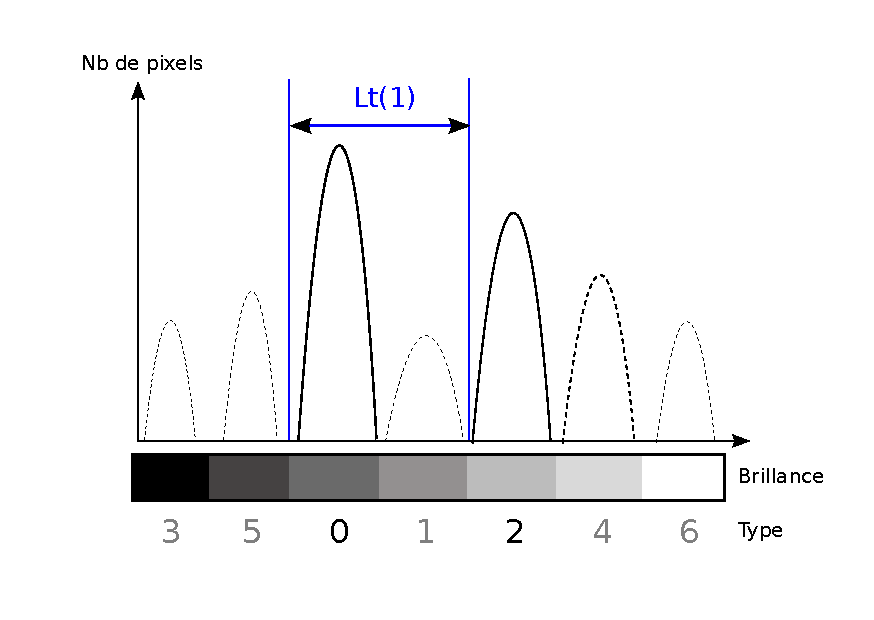
\includegraphics[trim= 0mm 5mm 0mm 5mm, clip, scale=0.3]{Formulation/figure/cas_1_histo.pdf}}	%trim=l b r t  width=0.5\textwidth, 
% 	      }\caption{Sous-ensemble non segmenté.}
%          \label{fig:contextual_info_rappel_ex}
% 	\end{figure}
% 	%%%%%%%%%%%%%%%%%%%%%%%%%%%%%%%%%%%%%%%%%%%%%%%%%%%

\begin{itemize}
\item Cas 4 : recherche du type $5$ sachant que les types 0, 2 et 4 ont été segmentés
\end{itemize}

	%%%%%%%%%%%%%%%%%%%%%%%%%%%%%%%%%%%%%%%%%%%%%%%%%%%
	\begin{figure}[!ht]	%trim=l b r t  width=0.5\textwidth,
	  \centering
	      \fbox{
		  \subfloat[Graphe $G_{T,t}$]{\label{fig:cas_4_graph_topo}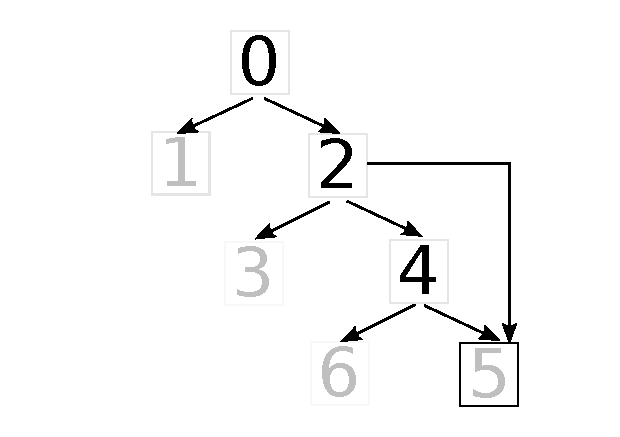
\includegraphics[trim= 20mm 5mm 0mm 5mm, clip, scale=0.4]{Formulation/figure/cas_4_graph_topo.pdf}}
		  %\subfloat[Image masquée]{\label{fig:cas_2_img}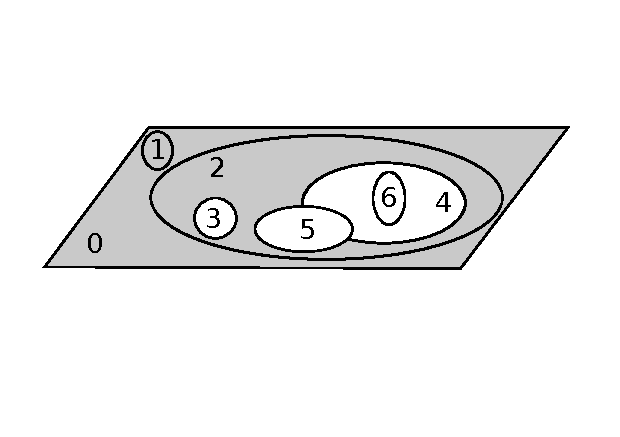
\includegraphics[trim= 8mm 20mm 10mm 5mm, clip, scale=0.5]{Formulation/figure/cas_2_img.pdf}}
		  \subfloat[Histogramme]{\label{fig:cas_4_histo}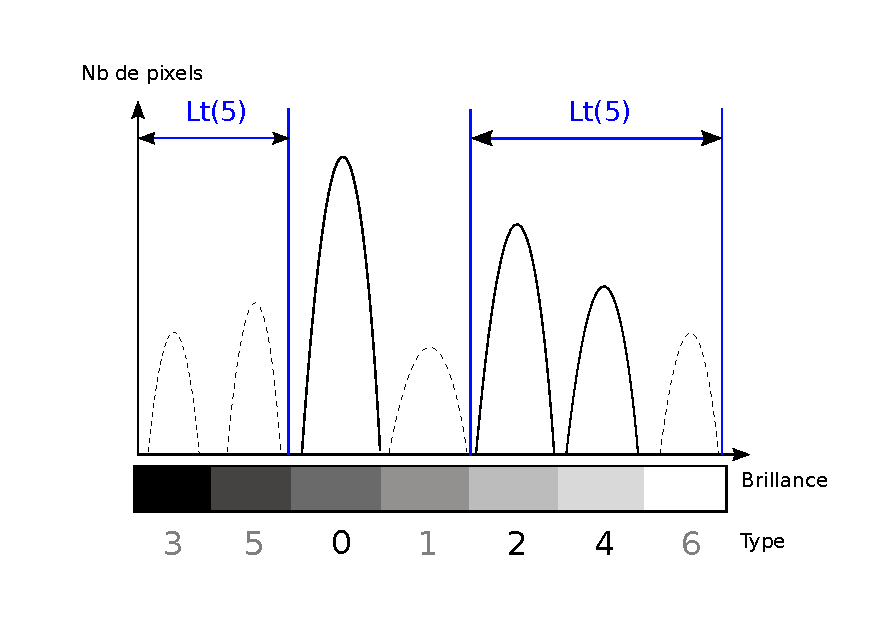
\includegraphics[trim= 0mm 10mm 0mm 5mm, clip, scale=0.4]{Formulation/figure/cas_4_histo.pdf}}
		  \subfloat[Graphe $G_{P,t}$]{\label{fig:cas_4_graph_photo}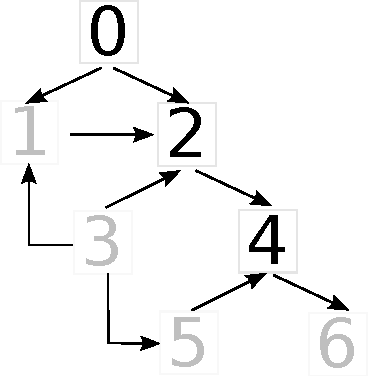
\includegraphics[trim= -10mm 0mm -10mm 0mm, clip, scale=0.4]{Formulation/figure/cas_4_graph_photo.pdf}}
	      }\caption{Sous-ensemble $L_t(5)$.}
         \label{fig:cas_4}
	\end{figure}
	%%%%%%%%%%%%%%%%%%%%%%%%%%%%%%%%%%%%%%%%%%%%%%%%%%%

	%%%%%%%%%%%%%%%%%%%%%%%%%%%%%%%%%%%%%%%%%%%%%%%%%%%
% 	\begin{equation}
% 	\begin{split}
% 	  L_t(5) = & \left( ( S \setminus S_t ) \cap G_{T}^\infty \left( G_{T,t}^{-1} \left( 5 \right) \right) \right) \cup G_{T,t}^{-1}(5) \\
% 		= & \left( \{1,3,5,6\} \cap G_T^{\infty}(\{ 2,4 \}) \right) \cup \{ 2,4 \} \\
% 		= & \left( \{1,3,5,6\} \cap \{ 3,4,5,6\}\right) \cup \{ 2,4 \} \\
% 		= & \left\{ 3,5,6 \right\} \cup \{ 2,4 \} \\
% 		= & \left\{ 3,5,6,2,4 \right\}
% 	\end{split}
% 	\end{equation}
	%%%%%%%%%%%%%%%%%%%%%%%%%%%%%%%%%%%%%%%%%%%%%%%%%%%

% 	%%%%%%%%%%%%%%%%%%%%%%%%%%%%%%%%%%%%%%%%%%%%%%%%%%%
% 	\begin{equation}
% 	\begin{split}
% 	  %L_t(5) = & \left( ( S \setminus S_t ) \cap G_{T}^\infty \left( G_T^{-1}(5) \setminus G_{T,t}^{-1} \left( 5 \right) \right) \right) \cup G_{T,t}^{-1}(5) \\
% 	 L_t(5) = & \left( \left( G_T(i) \ni G_{T,t}(u)  \right) \;|\; i \in G_{T,t}^{-1}(u) \right) \cup G_{T,t}^{-1}(5) \\
% 		= & \left( \left( G_T(i) \ni G_{T,t}(5)  \right) \;|\; i \in G_{T,t}^{-1}(\{ 2,4 \}) \right) \cup G_{T,t}^{-1}(5) \\
% 		= & \left( \left( G_T(i) \ni \{0,2,4\}  \right) \;|\; i \in G_{T,t}^{-1}(\{ 2,4 \}) \right) \cup G_{T,t}^{-1}(5) \\
% 		= & \left( \{1,3,5,6\} \cap G_T^{\infty}(\{ 2,4 \}) \right) \cup \{ 2,4 \} \\
% 		= & \left( \{1,3,5,6\} \cap \{ 3,4,5,6\}\right) \cup \{ 2,4 \} \\
% 		= & \left\{ 3,5,6 \right\} \cup \{ 2,4 \} \\
% 		= & \left\{ 3,5,6,2,4 \right\}
% 	\end{split}
% 	\end{equation}
% 	%%%%%%%%%%%%%%%%%%%%%%%%%%%%%%%%%%%%%%%%%%%%%%%%%%%

	%%%%%%%%%%%%%%%%%%%%%%%%%%%%%%%%%%%%%%%%%%%%%%%%%%%
	\begin{equation}
	\begin{split}
	  %L_t(5) = & \left( ( S \setminus S_t ) \cap G_{T}^\infty \left( G_T^{-1}(5) \setminus G_{T,t}^{-1} \left( 5 \right) \right) \right) \cup G_{T,t}^{-1}(5) \\
	 L_t(5) = & \left\{ i \in \left( G_T^{\infty}(G_{T,t}^{-1}(5)) \cap ( S \setminus S_t ) \right)\;|\; \left( G_{T,t}^{-1} (i) \cap G_{T,t}^{-1} (5) \neq \emptyset \right) \right\} \cup  G_{T,t}^{-1}(5)\\
		= & \left\{ i \in \left( \{3,6,5\} \cap \{1,3,5,6\} \right)\;|\; \left( G_{T,t}^{-1} (i) \cap \{2,4\} \neq \emptyset \right) \right\} \cup  \{2,4\} \\
		= & \left\{3,6,5\} \cup \{ 2,4 \right\} \\
	\end{split}
	\end{equation}
	%%%%%%%%%%%%%%%%%%%%%%%%%%%%%%%%%%%%%%%%%%%%%%%%%%%

	Parmi les types non segmentés, le type 1 n'a pas de prédécesseur commun avec ceux de $u$, il est donc exclu (fig.~\ref{fig:cas_4_graph_topo}). Il reste donc 3, 6 et 5 ainsi que les prédécesseurs de $u$ : 2 et 4 (second membre). L'ensemble trouvé $L_t(5) = \{3,6,5,2,4\}$ (fig.~\ref{fig:cas_4_histo}). Sa cardinalité $N_t(4) = \left|{L_t(5)}\right| = 5$.\vspace{1em}

	%%%%%%%%%%%%%%%%%%%%%%%%%%%%%%%%%%%%%%%%%%%%%%%%%%%
%	\begin{equation}
% 	\begin{split}
% 	 L_t(5) = & \left\{ ( S \setminus S_t ) \cap ( G_T^{\infty}(U) \setminus G_T^{\infty} (G_{T,t}^{+1}(U) ) ) \right\} \cup U \\
% 	  %L_t(5) = & \left( ( S \setminus S_t ) \cap G_{T}^\infty \left( G_{T,t}^{-1} \left( 5 \right) \right) \right) \cup G_{T,t}^{-1}(5) \\
% 		= & \left( \{1,3,5,6\} \cap \left( G_T^{\infty}(\{ 2,4 \}) \setminus G_T^{\infty} ( G_{T,t}^{+1}(\{ 2,4 \}) )  				\right) \right) \cup \{ 2,4 \} \\
% 		= & \left( \{1,3,5,6\} \cap \left( G_T^{\infty}(\{ 2,4 \}) \setminus G_T^{\infty} ( G_{T,t}^{+1}(\{2\}) \cup G_{T,t}^{+1}(\{4\}) )  	\right) \right) \cup \{ 2,4 \} \\
% 		= & \left( \{1,3,5,6\} \cap \left( G_T^{\infty}(\{ 2,4 \}) \setminus G_T^{\infty} ( \{4\} 		\cup \emptyset )  		\right) \right) \cup \{ 2,4 \} \\
% 		= & \left( \{1,3,5,6\} \cap \left( G_T^{\infty}(\{ 2,4 \}) \setminus \{6,5\} )  							\right) \right) \cup \{ 2,4 \} \\
% 	        = & \left( \{1,3,5,6\} \cap \left( \{ 3,4,5,6\}\setminus \{6,5\}									\right) \right) \cup \{ 2,4 \} \\
% 	        = & \left( \{1,3,5,6\} \cap \left( \{ 3,4\}												\right) \right) \cup \{ 2,4 \} \\
% 		= & \left\{ 3,2,4 \right\} (ERROR!!!)
% 	\end{split}
% 	\end{equation}
	%%%%%%%%%%%%%%%%%%%%%%%%%%%%%%%%%%%%%%%%%%%%%%%%%%%


	%%%%%%%%%%%%%%%%%%%%%%%%%%%%%%%%%%%%%%%%%%%%%%%%%%%
% 	\begin{equation}
% 		%N_t(u) = \operatorname{Card}\{X_t(i) \in R_t(u) \; \forall \;i\}
% 		%L_t(4) = \{i \in S \setminus S_t \;|\; X(i) \in R_t(4) \; AND \; G_{P,t}^{[4,2]} \}
% 		L_t(5) = \{i \in S \setminus S_t \;|\; X(i) \in R_t(5)\} \cup \{ G_{T,t}^{-1}(5) \}
% 		%nbClMax = \operatorname{Card}\{R_t(u)\}
% 		\label{eq:lobes_cas_4}
% 	\end{equation}
	%%%%%%%%%%%%%%%%%%%%%%%%%%%%%%%%%%%%%%%%%%%%%%%%%%%

	%L'ensemble des types non segmentés $S \setminus S_t = \{1,3,5,6\}$, restreint à $R_t(5)$, 1 est éliminé (fig.~\ref{fig:cas_4_graph_topo}). Le deuxième membre $G_{T,t}^{-1}(5) = \{2,4\}$, 4 étant déjà considéré par le premier membre, $L_t(5) = \{3,5,6,2,4\}$. Cet ensemble est représenté sur l'histogramme~\ref{fig:cas_4_histo}. Sa cardinalité $N_t(5) = \left|{L_t(5)}\right| = 5$.

	%(Réponse à une ancienne note\footnote{Ancienne formule: à quoi correspond $S(i)$ dans ($S(i) \in G_{T}^\infty( j \in G_{T,t}^{-1}(u) )$) ? C'est une erreur, $S(i)=>i$ et $j$ est un type appartenant à l'ensemble des prédécesseurs de $u$. Par contre, ta formulation semble plutôt correcte. Je précise tout du moins quelques petites choses: à discuter ensemble})
%\newpage
\begin{itemize}
\item Cas 5 : recherche du type $1$ sachant que les types 0 et 4 ont été segmentés
\end{itemize}

	%%%%%%%%%%%%%%%%%%%%%%%%%%%%%%%%%%%%%%%%%%%%%%%%%%%
	\begin{figure}[!ht]	%trim=l b r t  width=0.5\textwidth,
	  \centering
	      \fbox{
		  \subfloat[Graphe $G_{T,t}$]{\label{fig:cas_5_graph_topo}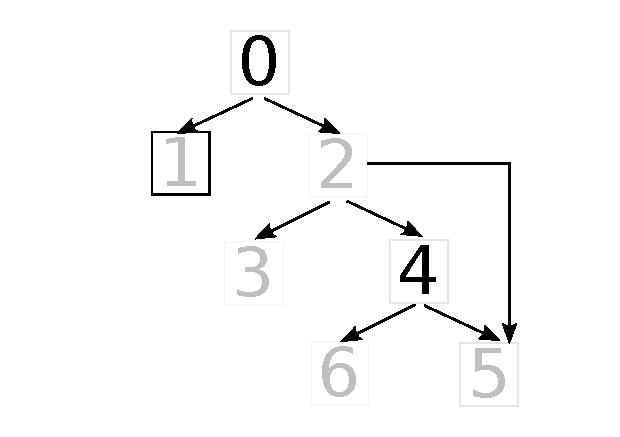
\includegraphics[trim= 20mm 5mm 0mm 5mm, clip, scale=0.4]{Formulation/figure/cas_5_graph_topo.pdf}}
		  %\subfloat[Image masquée]{\label{fig:cas_2_img}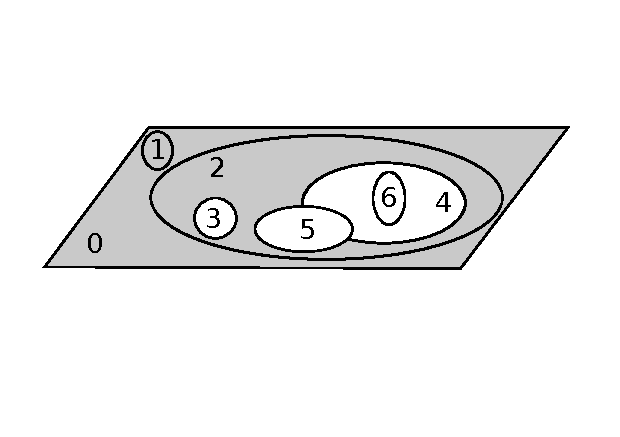
\includegraphics[trim= 8mm 20mm 10mm 5mm, clip, scale=0.5]{Formulation/figure/cas_2_img.pdf}}
		  \subfloat[Histogramme]{\label{fig:cas_5_histo}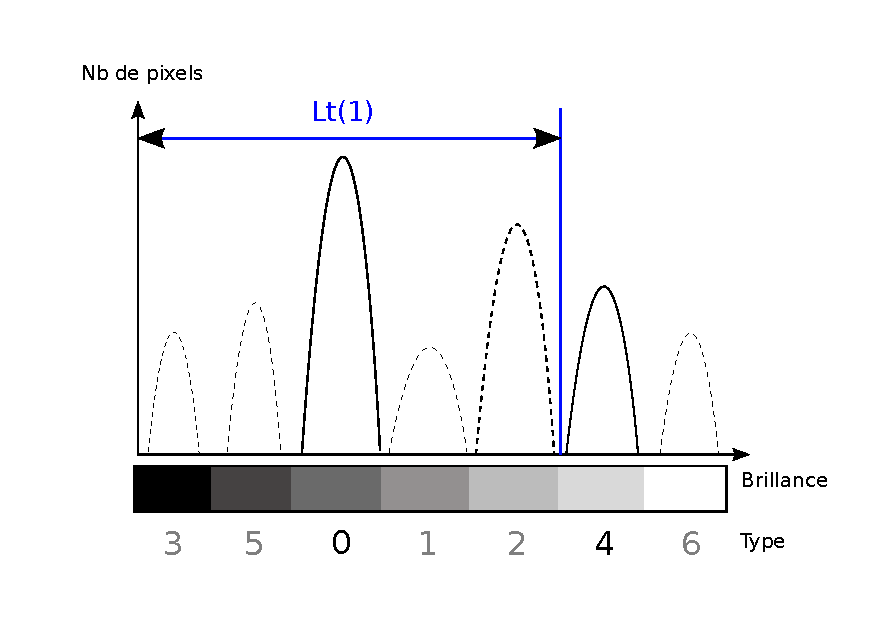
\includegraphics[trim= 0mm 10mm 0mm 5mm, clip, scale=0.4]{Formulation/figure/cas_5_histo.pdf}}
		  \subfloat[Graphe $G_{P,t}$]{\label{fig:cas_5_graph_photo}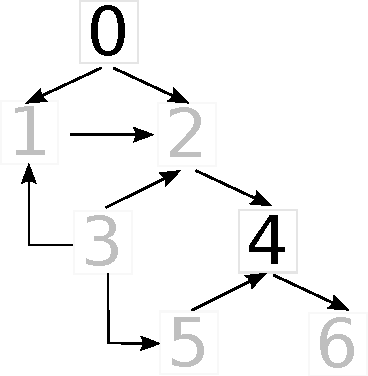
\includegraphics[trim= -10mm 0mm -10mm 0mm, clip, scale=0.4]{Formulation/figure/cas_5_graph_photo.pdf}}
	      }\caption{Sous-ensemble $L_t(5)$.}
         \label{fig:cas_5}
	\end{figure}
	%%%%%%%%%%%%%%%%%%%%%%%%%%%%%%%%%%%%%%%%%%%%%%%%%%%


	%%%%%%%%%%%%%%%%%%%%%%%%%%%%%%%%%%%%%%%%%%%%%%%%%%%
	\begin{equation}
	\begin{split}
	 L_t(1) = & \left\{ i \in \left( G_T^{\infty}(G_{T,t}^{-1}(1))  \cap ( S \setminus S_t ) \right) \;|\; \left( G_{T,t}^{-1} (i) \cap G_{T,t}^{-1} (1) 	\neq \emptyset \right) \right\} \cup  G_{T,t}^{-1}(1)	\\
		= & \left\{ i \in \left( 	\{1,2,3,4,5,6\} 	\cap 	\{1,2,3,6,5\}	 \right) \;|\; \left( G_{T,t}^{-1} (i) \cap 	\{0\} 		\neq \emptyset \right) \right\} \cup  	\{0\}		\\
		= & \left\{ 1,2,3,5 \right\}																			\cup  	\{0\}
	\end{split}
	\end{equation}
	%%%%%%%%%%%%%%%%%%%%%%%%%%%%%%%%%%%%%%%%%%%%%%%%%%%

	Ici on teste le cas où les types n'ont pas été segmentés suivant l'ordre topologique. La formule reste robuste car on obtient bien l'ensemble des prédécesseurs de 1 avec leurs successeurs non segmentés à l'exception de 6 puisque il a pour prédécesseur $\{4\} \neq \{0\} = G_{T,t}^{-1}(1)$.

\begin{comment}

	%Une amélioration pourrait être que $L_t(u)$ soit l'union de l'ensemble des successeurs $i$, non actifs ($i \in S \setminus S_t$), de chacun des prédécesseurs directs "actifs" (\in $S_t$) de $u$ et des prédécesseurs de $u$ eux-mêmes.%l'ensemble des types $i$ non actifs ($i \in S \setminus S_t$) qui sont inclus dans
 	
% 	Une amélioration de $L_t(u)$ pourrait être, pour un élément $i$ issu des prédécesseurs de $u$ ($i\in G_{T,t}^{-1}(u)$), l'union de l'ensemble des successeurs non segmentés ($G_T^{\infty}(i) \cap \{S \setminus S_t\}$) et des prédécesseurs de $u$ eux-mêmes ($G_{T,t}^{-1}(u)$).%.    (i.e. éléments de $S \setminus S_t$) et des prédécesseurs de $u$ (i.e. $G_{T,t}^{-1}(u)$).   soit l'union de l'ensemble des successeurs $i$, non actifs ($i \in S \setminus S_t$), de chacun des prédécesseurs directs "actifs" de $u$ ($G_{T,t}^{-1}(u)$) et des prédécesseurs de $u$ eux-mêmes ($G_{T,t}^{-1}(u)$). %l'ensemble des types $i$ non actifs ($i \in S \setminus S_t$) qui sont inclus dans
% 
% 	%{\bf L'ensemble des prédécesseurs directs "actifs" de $u$ est: $G_{T,t}^{-1}(u)$}
% 
% 	L'union de l'ensemble de ses successeurs non segmentés d'un type $k$ ($G_T^{\infty}(k) \cap \{S \setminus S_t\}$) peut être également noté $\{ k\in S \setminus S_t|\; k \in G_T^{\infty}(i)\}$.
% 
% 	%{\bf Pour un élément $i$ donné de ces prédécesseurs (i.e. $i\in G_{T,t}^{-1}(u)$), l'ensemble des successeurs non valides (i.e. éléments de $S \setminus S_t$) peut être noté: $G_T^{\infty}(i) \cap \{S \setminus S_t\}$ ou $\{ k\in S \setminus S_t|\; k \in G_T^{\infty}(i)\}$.}
% 
% 	On peut en déduire la formule suivante pour $L_t(u)$, sans explicitement utilisé la ROI:
% 
% \begin{equation}
% L_t(u) =  \left(\bigcup_{i\in G_{T,t}^{-1}(u)} \{ k\in S \setminus S_t|\; k \in G_T^{\infty}(i)\} \right) \cup \left\{ G_{T,t}^{-1}(u) \right\}
% \end{equation}
% 
% %{\bf On peut introduire la notion de prédécesseurs-successeurs d'un ensemble de noeuds, e.g. $G_{T}^\infty(G_{T,t}^{-1}(u) )$ (à introduire dans le glossaire des notations comme étant l'union des prédécesseurs-successeurs de chacun des éléments de l'ensemble).}
% La formule précédente se simplifie :
% \begin{equation}
% L_t(u) =  \{ i\in S \setminus S_t|\; i \in G_T^{\infty}(G_{T,t}^{-1}(u))\} \cup G_{T,t}^{-1}(u)
% \end{equation}
% 
% C'est à dire :
% 
% \begin{equation}
% L_t(u) = \left\{ ( S \setminus S_t ) \cap  G_T^{\infty}(G_{T,t}^{-1}(u)) \right\} \cup G_{T,t}^{-1}(u)
% \end{equation}
% 

%{\bf L'ensemble de recherché est $\{i \in S \setminus S_t |\; dsqf\}$ prédécesseurs directs "actifs" de $u$ est: $G_{T,t}^{-1}(u)$}

% \begin{itemize}
% \item Application au cas 3:
% \end{itemize}
% \begin{equation}
% L_t(4) = \left( ( S \setminus S_t ) \cap  G_T^{\infty}(G_{T,t}^{-1}(4)) \right) \cup G_{T,t}^{-1}(4)
% \end{equation}
% \begin{equation}
% L_t(4) = \left(\{1,4\} \cap G_T^{\infty}(\{2\})\right) \cup \{ 2 \}
% \end{equation}
% \begin{equation}
% L_t(4) =   \left(\{1,4\} \cap \{ 3,4,5,6\}\right) \cup \{ 2 \}
% \end{equation}
% \begin{equation}
% L_t(4) =   \{ 4\} \cup \{ 2 \} =   \{ 4,2 \}
% \end{equation}


% \begin{equation}
% L_t(5) = \left( ( S \setminus S_t ) \cap  G_T^{\infty}(G_{T,t}^{-1}(5)) \right) \cup G_{T,t}^{-1}(5)
% \end{equation}
% \begin{equation}
% L_t(5) = \left( \{1,3,5,6\}  \cap G_T^{\infty}(\{2,4\}) \right) \cup \{2,4\}
% \end{equation}
% \begin{equation}
% L_t(5) =  \left( \{1,3,5,6\} \cap \{3,4,5,6\} \right) \cup \{2,4\}
% \end{equation}
% \begin{equation}
% L_t(5) =  \{3,5,6\} \cup \{2,4\} = \{3,5,6,2,4\}
% \end{equation}





%($S(i) \in G_{T}^\infty( j \in G_{T,t}^{-1}(u) )$). Ainsi que le prédécesseur lui même ($G_{T,t}^{-1}(u)$). %Pour que cette amélioration s'applique dans le cas où $u$ a plusieurs prédécesseurs direct actifs on considérera l'union de ces prédécesseurs ($\bigcup{ G_{T,t}^{-1}(u)}$).

% potientielle à fournir sur $L_t$ serait de plus dépendre des régions de l'image dans la formulation, mais seulement des noeuds du graphe (facilitera également l'implémentation). La formule actuelle devra être conservée comme formule intermédiaire permettant de mieux comprendre la démarche par rapport à la ROI.}
% {\bf Ci-après: ta version : je l'ai laissé temporairement: peut-être à enlever si pertinent après validation ensemble.}
% \begin{itemize}
% \item Application au cas 3:
% \end{itemize}
% 	%%%%%%%%%%%%%%%%%%%%%%%%%%%%%%%%%%%%%%%%%%%%%%%%%%%
% 	\begin{equation}
% 		L_t(u) = \left\{i \in S \setminus S_t \;|\; i \in G_{T}^\infty \left( j \in G_{T,t}^{-1}\left( u \right) \right) \right\} \cup \left\{ G_{T,t}^{-1}(u) \right\}
% 		\label{eq:new}
% 	\end{equation}
% 	%%%%%%%%%%%%%%%%%%%%%%%%%%%%%%%%%%%%%%%%%%%%%%%%%%%
% 	
% 	Avec :
% 
% 	\begin{itemize}
% 	  \item $S \setminus S_t = \{1,4\}$
% 	  \item $G_{T,t}^{-1}\left( 4 \right) = \{2\}$
% 	  \item $G_{T}^\infty \left( 2 \right)=\{3,4,6,5\}$
% 	\end{itemize}
% 
% 	%%%%%%%%%%%%%%%%%%%%%%%%%%%%%%%%%%%%%%%%%%%%%%%%%%%
% 	\begin{equation}
% 	\begin{split}
% 	  L_t(4) = & \left\{ i \in S \setminus S_t \;|\; i \in G_{T}^\infty \left( j \in G_{T,t}^{-1}\left( 4 \right) \right) \} \cup \{ G_{T,t}^{-1}(4) \} \right. \\
% 		= & \left\{ i \in \{1,4\} \;|\; i \in \{3,4,6,5\} \cup \{ 2 \} \right. \\
% 		= & \left.\{ 4, 2 \right\}
% 	\end{split}
% 	\end{equation}
% 	%%%%%%%%%%%%%%%%%%%%%%%%%%%%%%%%%%%%%%%%%%%%%%%%%%%
% 
% \begin{itemize}
% \item Application au cas 4:
% \end{itemize}
% 	Application de la formule améliorée :
% 	%%%%%%%%%%%%%%%%%%%%%%%%%%%%%%%%%%%%%%%%%%%%%%%%%%%
% 	\begin{equation}
% 	\begin{split}
% 	  L_t(5) = &\left. \{ i \in S \setminus S_t \;|\; i \in G_{T}^\infty \left( j \in G_{T,t}^{-1}\left( 5 \right) \right) \} \cup \{ G_{T,t}^{-1}(5) \} \right. \\
% 		= & \left. \{ i \in \{1,3,6,5\} \;|\; i \in \{3,4,6,5\} \cup \{ 4,2 \} \right. \\
% 		= & \left. \{ 3,6,5,4,2\} \right. \\
% 		  & \left. \right. \\
% 	  N_t(5)= & \left. \operatorname{card}\{L_t(5)\} \right. \\
% 		= & \left. \operatorname{card}\{3,6,5,4,2\} \right. \\
% 		= & \left. 5 \right.
% 	\end{split}
% 	\end{equation}
% 	%%%%%%%%%%%%%%%%%%%%%%%%%%%%%%%%%%%%%%%%%%%%%%%%%%%
% 
% 	Avec :
% 
% 	\begin{itemize}
% 	  \item $S \setminus S_t = \{1,3,6,5\}$
% 	  \item $G_{T,t}^{-1}\left( 5 \right) = \{4,2\}$
% 	  \item $G_{T}^\infty \left( 4 \right)=\{6,5\}$
% 	  \item $G_{T}^\infty \left( 2 \right)=\{3,4,6,5\}$
% 	\end{itemize}
\end{comment}

%\newpage

% \newpage
% \begin{itemize}
% \item Cas 7 : recherche du type $6$ sachant que les types 0, 2, 4 et 6 ont été segmentés et que tous les types 6 sont segmentés : 
% \end{itemize}

	%A venir...\hspace{1em}
	%\textit{Dans le cas de la multiplicité, cela se transformera peut-être en un intervalle, i.e. un nombre min et max de lobe, permettant tout de même d'apporter des informations sur le nombre de classes min et max à utiliser pour la recherche de lobe avec gaussian mixture... le travail deviendra intéressant: il y aura une recherche d'un nombre classe optimal entre un min et un max (fonction de l'erreur d'estimation)... On verra plus tard comment ajuster la formule 1.3 pour qu'elle reste valable dans les deux cas.}


%     \subsubsection*{Caractère optionnel des types (0 ou 1)}

%	L'aspect optionnel des types dans l'image est dû aux type de structures (e.g.pathologiques). Si des types sont considérés comme optionnels, l'ensemble $L_t(u)$ deviendra de taille variable et influencera directement $N_t(u)$. On pourra dire que $N_t(u) \in \left[a, b\right]$ avec $a$ et $b$ les valeurs minimale et maximale de $N_t(u)$.
	%Appliqué à notre cas : $N_t(6) = \left[ \min{ \operatorname{card}\{L_t(6)\}}, \max{\operatorname{card}\{L_t(6)\}} \right] = \left[1, 3 \right]$.

\newpage
      \subsection{Identification des lobes}
	Nous identifions les lobes (correspondant aux classes de l'image) présentes dans l'image pour pouvoir optimiser le fenêtrage de la structure recherchée. L'identification consiste en l'ordonnancement des lobes de l'ensemble $L_t$ en fonction de leur intensité lumineuse. Dans cette étude, et sous l'hypothèse d'une distribution des intensités selon un loi normale, ``plus sombre'', se traduira par la moyenne (de la gaussienne) des intensités de $i$ est inférieure à la moyenne des intensités de $j$. On s'appuie sur les relations photométriques inter-types que l'on représente par un graphe (voir fig.~\ref{fig:info_photo_graph}) dont des arcs orientés signifient ``plus sombre que''. On utilise ensuite l'opérateur \texttt{ord} qui comparera les relations photométriques inter-type jusqu'à l'obtention d'une suite de types ordonnés par intensité moyenne croissante. On exprime cette opération par :


	%%%%%%%%%%%%%%%%%%%%%%%%%%%%%%%%%%%%%%%%%%%%%%%%
% 	\begin{equation}
% 		%N_t(u) = \operatorname{Card}\{X_t(i) \in R_t(u) \; \forall \;i\}
% 		L_{t,i}(u) = \operatorname{ord} \{ L_t(u) \} \; \forall \; i,j \in L_t(u)
% 		%nbClMax = \operatorname{Card}\{R_t(u)\}
% 		\label{eq:lobes}
% 	\end{equation}

	\begin{equation}
		O_t(u) = \operatorname{ord} \{ L_t(u) \} = \{ L_{t,i}(u) \; |\; i \in \{0,...,N_t-1\} \}
		\label{eq:8}
	\end{equation}
	%%%%%%%%%%%%%%%%%%%%%%%%%%%%%%%%%%%%%%%%%%%%%%%%

	Cet ensemble est ordonné, ce qui signifie que, $\forall (i,j) \in \{0,...,N_t-1\}^2\; |\; \left( L_{t,i}\left(u\right),L_{t,j}\left(u\right)\right) \in \left( O_t\left(u\right), L_{t,i}\left(u\right) < L_{t,j}\left(u\right)\right)$ \footnote{La relation $\in O, L < L$ ne me semble pas claire, est-ce vraiment la représentation standard pour un ensemble ordonné et sont opérateur? Ne doit-on pas plutôt utiliser des accolades quand on parle d'ensemble?} :
	%({\bf finalement, il est peut-être préférable de retirer la notion de comparaison entre région (i.e. la formule $X(i)< X(j)$ présente dans la précédente version), car il peut y avoir ambiguïté avec une relation de taille entre les régions. Bilan: ce qui suit me paraît suffisant})
	\begin{itemize}
		\item
		En terme d'image: la région $X(i)$ est plus sombre que la région $X(j)$
		\item
		En terme de graphe: le noeud $i$ est prédécesseur de $j$ dans le graphe $G_{P} \Rightarrow i \in G_{P,t}^{-\infty}(j)$
	\end{itemize}

	%Remarque à placer quelque part: la notion "$i$ est plus sombre que la région $j$" signifie que, globalement, la région $i$ est plus sombre que la région $j$. "Globalement" car certains point de la région $i$ peuvent être plus clairs que certains autres points de la région $j$ (e.g. récouvrement des lobes). Dans cette étude, et sous l'hypothèse d'une distribution des intensités selon un loi normale, "plus sombre" se traduira par la moyenne (de la gaussienne) des intensités de $i$ est inférieure à la moyenne des intensités de $j$.

	%%%%%%%%%%%%%%%%%%%%%%%%%%%%%%%%%%%%%%%%%%%%%%%%%%%
	\begin{figure}[!ht]
	  \centering
	      \fbox{
		  \subfloat[Graphe $G_{P_t}$]
		  {\label{fig:info_photo_graph}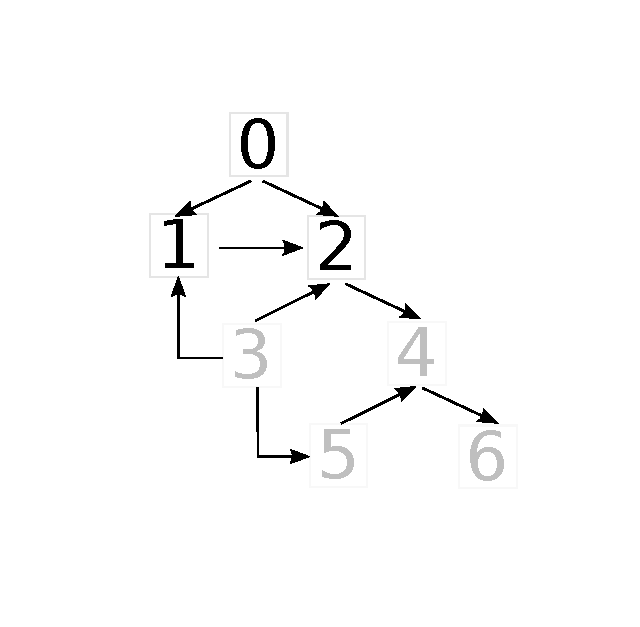
\includegraphics[trim= 0mm 0mm 0mm 5mm, clip, scale=0.3]{Formulation/figure/info_photo_a_priori.pdf}}
		  \subfloat[Lobes identifiés]
		  {\label{fig:ident_histo}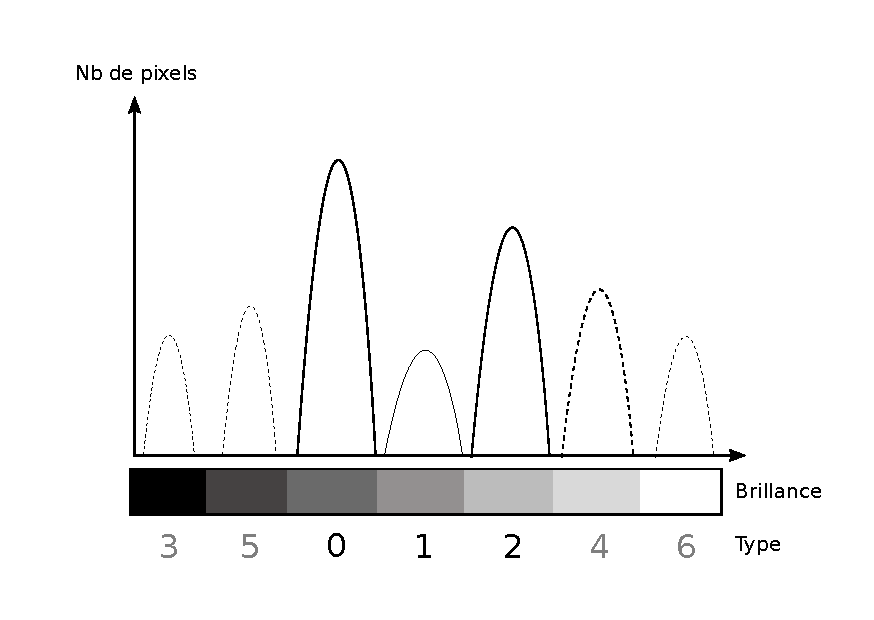
\includegraphics[trim= 0mm 5mm 0mm 5mm, clip, scale=0.3]{Formulation/figure/ident_histo.pdf}}	%trim=l b r t
	      }\caption{Exemple de représentation des informations photométriques ($G_{P,t}$) correspondant au cas n$^{\circ}$2 énoncé plus haut.}
         \label{fig:info_photo_a_priori}
	\end{figure}
	%%%%%%%%%%%%%%%%%%%%%%%%%%%%%%%%%%%%%%%%%%%%%%%%%%%

	Appliqué au cas n$^{\circ}$2, $O_t(3)$ compare la relation photométrique entre les types de l'ensemble $L_t(3) = \{2,3,4,5,6\}$ deux à deux, c.a.d. chaque type {\bf $i\in L_t(3)$} va être comparé à un autre type $j\in L_t(3)$ itérativement. 
	
	Selon~\ref{fig:info_photo_graph}, 2 est plus clair que 3 qui est plus sombre que 5 et ainsi de suite $\Rightarrow O_t(3) = \{3,5,2,4,6\}$. Le premier lobe de l'histogramme ~\ref{fig:ident_histo} est donc identifié comme étant de type 3, le second de type 5 et ainsi de suite sachant que 0 et 1 sont exclut de $L_t(3)$.

\newpage
	\section{Discussion: limites et perspectives}

	Dans la formulation dédiée à la photométrie (section~\ref{sec:inf_and_photo}), nous avons considéré des régions avec une multiplicité de 1. Cette hypothèse simplificatrice signifie que nous avons ignoré les situations suivantes:
\begin{itemize}
\item le caractère optionnel d'une région (e.g. une tumeur peut être absente bien que représentée dans le graphe) ;
\item le caractère multiple d'une région : ceci peut notamment concerner le cas de tumeurs multiples, chacune d'elles étant segmentée à une étape différente du processus d'analyse ;
\item le cas où une région $A$ contient des sous-régions dont l'union occupe toute la région $A$ : il n'y alors aucune classe (lobe de l'histogramme) qui correspond spécifquement à la région $A$.
\end{itemize}\vspace{1em}

	Contrairement au cas de la ROI \citep[Fasquel]{Fasquel2006}, cet aspect a un impact sur les déductions faites par le moteur d'inférence comme le nombre de classes. Ce choix est justifié par le fait que la formalisation proposée apparaît, comme constaté dans les sections précédentes, relativement complexe, malgré cette hypothèse simplificatrice. Ceci justifie donc de débuter l'étude dans un cas simple même si l'hypothèse simplificatrice peut s'avérer très limitante d'un point de vue applicatif (e.g. cas précédemment cité des tumeurs). 

	L'élimination de cette hypothèse nécessite de poursuivre l'étude, ce qui aurait probablement pour conséquence de modifier le formalisme présenté, notamment concernant la détermination du nombre de classe qui conduirait non plus à une valeur exacte mais probablement à un intervalle (e.g. selon qu'une tumeur est présente ou non, le nombre de classe peut varier entre un minimum et un maximum).
	
	Nous avons fait le choix d'évaluer cette première phase de l'étude en priorité afin d'en discuter des bénéfices, plutôt que d'étendre davantage le formalisme. Le bilan de cette partie est que la formalisation n'est pas triviale, contrairement à ce que l'on pourrait intuitivement penser en première approche, et qu'une étude des bénéfices semble pertinente avant de légitimer un effort de formalisation supplémentaire.

	Néanmoins, avant de détailler les études relatives à cette évaluation, nous présentons succinctement quelques pistes qui pourraient être envisagées dans le cas d'une multiplicité supérieure à 1. Le caractère optionnel (multiplicité 0) n'ayant pas été abordé.
	
%{\bf Ce travail a, pour le moment été limité où une région est supposée présente dans l'image, sans caractère optionnel. En effet, on peut considérer qu'un noeud du graphe peut être associé à une ou plusieurs régions (région "multiple"), segmentées à des étapes distinctes du processus d'analyse. Dans le cadre d'images médicales, ceci peut s'apparenter à la présence de plusieurs tumeurs, pouvant être segmentées à différentes étapes du processus d'analyse. Nous considérerons ci-après le cas d'une multiplicité égale à 1 et ensuite le cas d'une multiplicité supérieure à 1. Nous faisons l'hypothèse simplificatrice que les propriétés photométriques associées à une noeud sont constantes, même en cas de multiplicité supérieure à 1. D'un point de vue pratique, ceci signifie que différentes régions associées à un même noeud auront par exemple la même intensité moyenne et le même écart-type. 

%Le cas non traité ici concerne une multiplicité nulle, relatif à une région dont la présence n'est pas certaine (e.g. une tumeur). Cet aspect pourrait faire l'objet d'une étude complémentaire.}


%		Le moteur d'inférence agit comme une interface entre les informations à priori (à renseigner manuellement) et leur traitement selon le formalisme définis ci-dessus. Dans la suite du document, on l'utilisera comme un système d'information qui renvoi une réponse en fonction de ce qu'on lui infère. 

 
%      \subsection{A conserver ? Cas de multiplicité de 1 à N types similaires}	% de $\mathbb{N}$}
	Une piste envisageable repose sur l'ajout d'un attribut (nous le noterons $M$) à chaque noeud du graphe, spécifiant la multiplicité potentielle d'une région. Une limitation de cette approche concerne l'élément quantitatif introduit dans la représentation des connaissances, sachant que nous privilégions une représentation des connaissances non quantitative dans la méthode proposée. Dans ce contexte, nous ferons l'hypothèse que les différentes régions d'une même classe ($M$>1) présentent les mêmes propriétés photométriques.\\

%	Ici nous considérons que tous les types $\in S$ peuvent avoir un caractères multiples $M(i)$ (e.g. pathologie identique et multiple). La multiplicité, notée $M$ ici, fait partie des connaissances topologiques à priori. Une multiplicité de $N$, signifie que chaque type peut apparaître plusieurs fois dans l'image, il peut donc y avoir deux ou plusieurs tumeurs hépatiques par exemple. On pourra interpréter cette information comme la présence de deux types photométriquement identiques (sous l'hypothèse qu'ils ont la même distribution) et spatialement différents. 

%Nous rappelons que ce cas peut par exemple être rencontré lorsque, après la segmentation de la région d'intérêt d'un type $u$, un nouveau type identique à $u$ apparaîtra dans l'histogramme de l'image dans le même intervalle d'intensité que $u$. 

%%%%%%%%%%%%%%%%%%%%%%%%%%%%%%%%%%%%%%%%%%%%%%%%%%%%%%%%%%%%%%%%%%%%%%%%%%%%%%%%%%%%%%%%%%%%%%%%%%%%%%%%%%%%%%%%%%%%%%%%%%%%%
%														MULTIPLICITE														%
%%%%%%%%%%%%%%%%%%%%%%%%%%%%%%%%%%%%%%%%%%%%%%%%%%%%%%%%%%%%%%%%%%%%%%%%%%%%%%%%%%%%%%%%%%%%%%%%%%%%%%%%%%%%%%%%%%%%%%%%%%%%%

%{\bf CI-DESSOUS: NE PAS LE METTRE DANS LA PRESENTATION POUR LE MOMENT CAR IL N'EST PAS CERTAIN QUE CE SOIT CONSERVÉ.\\}

%Ceci signifie que nous devons donc inclure, au sous-ensemble $L_t(u)$ présenté précédemment, les types déjà segmentés $\in S_t$ qui ont une multiplicité $>$ 1 car ils seront présent dans l'image. Le niveau de multiplicité $M(i)$ devra être décrémenté à chaque segmentation du type $u$ pour converger vers la forme précédente de $L_t(u)$ lorsque il sera égal à 0 ou 1.\\
%	Complétons le sous-ensemble $L_t$ en ajoutant les types déjà segmentés ayant une multiplicité $>$ 1 pour considérer les lobes résiduelles après la segmentation :

%	%%%%%%%%%%%%%%%%%%%%%%%%%%%%%%%%%%%%%%%%%%%%%%%%
%	\begin{equation}
%	  \begin{split}
%	    Lm_t(u) = & L_t(u)  \cup  \left\lbrace i \in G_{T,t}^{\infty} \left(G_{T,t}^{-1} \left(u \right) \right) | M(i) > M_t(i) \right\rbrace
%	  \end{split}
%	  \label{eq:subset_multiple_2_n}
%	\end{equation}\vspace{1em}
%	%%%%%%%%%%%%%%%%%%%%%%%%%%%%%%%%%%%%%%%%%%%%%%%%

%\begin{itemize}
%\item Cas 1 : recherche du type $6$ sachant que les types 0, 2 et 4 ont été segmentés et qu'il y a au moins deux structures non segmenté de type 6 présentent dans l'image ($M(6) > 2$) :
%\end{itemize}

%	%%%%%%%%%%%%%%%%%%%%%%%%%%%%%%%%%%%%%%%%%%%%%%%%%%%
%	\begin{figure}[!ht]	%trim=l b r t  width=0.5\textwidth,
%	  \centering
%	      \fbox{
%		  \subfloat[Graphe $G_T,t$]{\label{fig:cas_1_n_graph_topo}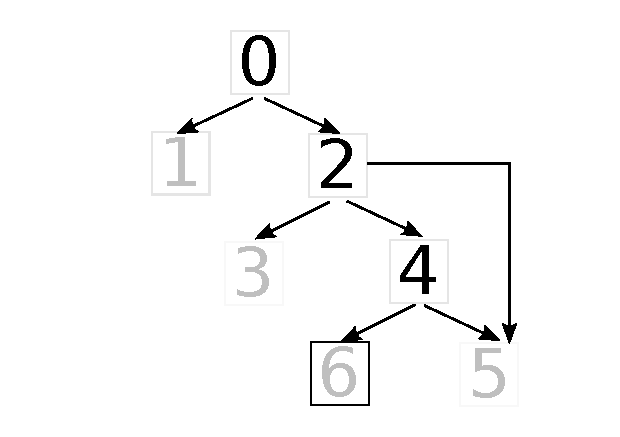
\includegraphics[trim= 20mm 5mm 0mm 5mm, clip, scale=0.4]{Formulation/figure/cas_1_n_graph_topo.pdf}}
%		  \subfloat[Image synthétique]{\label{fig:cas_1_n_img}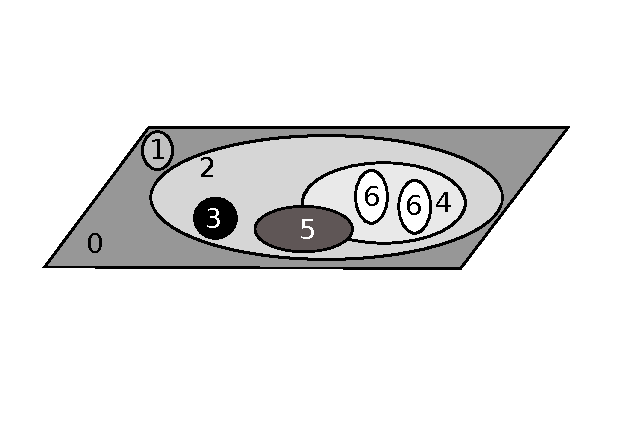
\includegraphics[trim= 5mm 20mm 5mm 5mm, clip, scale=0.5]{Formulation/figure/cas_1_n_img.pdf}}
%		  \subfloat[Histogramme]{\label{fig:cas_1_n_histo}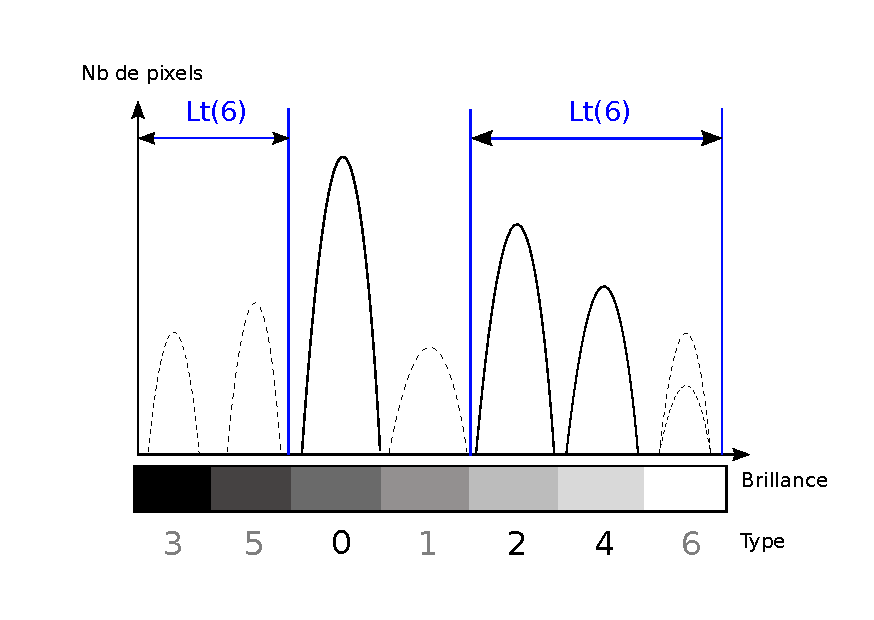
\includegraphics[trim= 0mm 10mm 0mm 5mm, clip, scale=0.5]{Formulation/figure/cas_1_n_histo.pdf}}
%		  %\subfloat[Graphe $G_{P,t}$]{\label{fig:cas_4_graph_photo}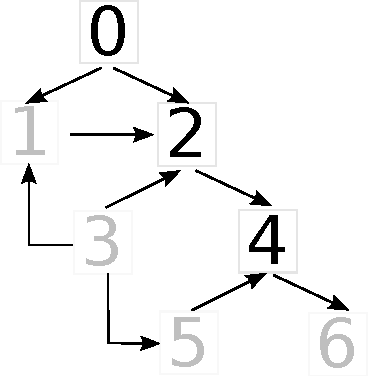
\includegraphics[trim= -10mm 0mm -10mm 0mm, clip, scale=0.4]{Formulation/figure/cas_4_graph_photo.pdf}}
%	      }\caption{Sous-ensemble $L_t(6)$.}
%         \label{fig:cas_1_n}
%	\end{figure}
%	%%%%%%%%%%%%%%%%%%%%%%%%%%%%%%%%%%%%%%%%%%%%%%%%%%%

%	%%%%%%%%%%%%%%%%%%%%%%%%%%%%%%%%%%%%%%%%%%%%%%%%%%%
%	\begin{equation}
%	\begin{split}
%	  Lm_t(6) = & L_t(6)  \cup  \left\lbrace i \in G_{T,t}^{\infty} \left(G_{T,t}^{-1}(u) \right) | M(i) > M_t(i) \right\rbrace \\
%		= & \{5,4,6\}  \cup  \left\lbrace i \in \{\emptyset\} | 2 > 0 \right\rbrace \\
%		= & \{5,4,6\}  \cup  \{6\} \\
%	\end{split}
%	\end{equation}
%	%%%%%%%%%%%%%%%%%%%%%%%%%%%%%%%%%%%%%%%%%%%%%%%%%%%

%	Le nombre de lobes $N_t(6) = \left|{L_t(6)}\right| = \left|{5,6,4}\right| = 3$. Ici le type 6 peut être multiple sans changer le résultat car il n'est pas segmenté donc déjà inclus dans $L_t(6)$. Notons que dans l'histogramme~\ref{fig:cas_1_n_histo} tous les types 6 sont confondus sous un unique lobe à ce stade de la segmentation.\vspace{1em}

%\begin{itemize}
%\item Cas 2 : recherche du type $6$ sachant que les types 0, 2, 4 et 6 ont été segmentés une fois ($M_t(6)=1$) et que 6 a une multiplicité de 2 ($M(6)=2$) dans l'image : 
%\end{itemize}

%	%%%%%%%%%%%%%%%%%%%%%%%%%%%%%%%%%%%%%%%%%%%%%%%%%%%
%	\begin{figure}[!ht]	%trim=l b r t  width=0.5\textwidth,
%	  \centering
%	      \fbox{
%		  \subfloat[Graphe $G_T,t$]{\label{fig:cas_2_n_graph_topo}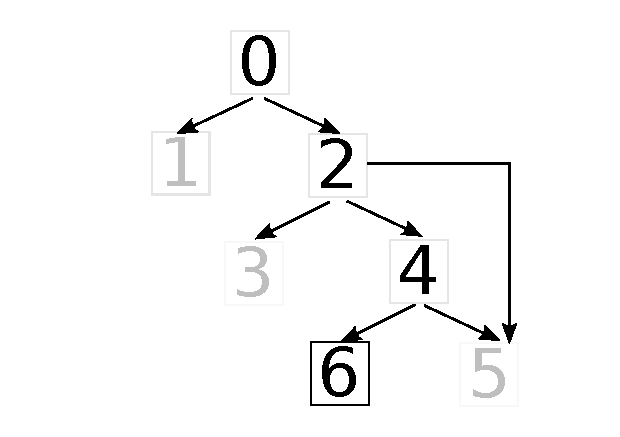
\includegraphics[trim= 20mm 5mm 0mm 5mm, clip, scale=0.4]{Formulation/figure/cas_2_n_graph_topo.pdf}}
%		  \subfloat[Image synthétique]{\label{fig:cas_2_n_img}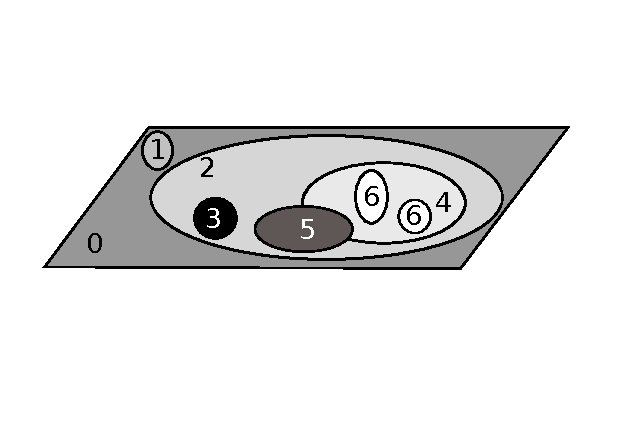
\includegraphics[trim= 5mm 20mm 5mm 5mm, clip, scale=0.6]{Formulation/figure/cas_2_n_img.pdf}}
%		  \subfloat[Histogramme]{\label{fig:cas_2_n_histo}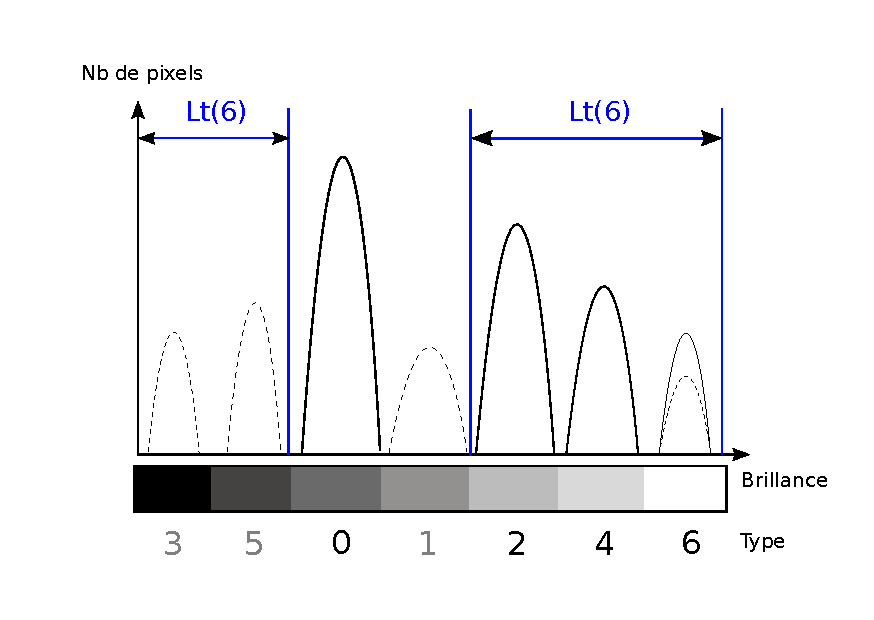
\includegraphics[trim= 0mm 10mm 0mm 15mm, clip, scale=0.5]{Formulation/figure/cas_2_n_histo.pdf}}
%	      }\caption{Sous-ensemble $L_t(6)$.}
%         \label{fig:cas_2_n}
%	\end{figure}
%	%%%%%%%%%%%%%%%%%%%%%%%%%%%%%%%%%%%%%%%%%%%%%%%%%%%

%	%%%%%%%%%%%%%%%%%%%%%%%%%%%%%%%%%%%%%%%%%%%%%%%%%%%
%	\begin{equation}
%	\begin{split}
%	  Lm_t(6) = & L_t(6) \cup \left\lbrace i \in G_{T,t}^{\infty} \left({ G_{T,t}^{-1} (6) }\right) | M(i) > M_t(i) \right\rbrace \\ 
%		= & \{5,4\} \cup \left\lbrace i \in \{6\} \;|\; 2 > 1 \right\rbrace \\ 
%		= & \{5,4,6\}
%	\end{split}
%	\end{equation}
%	%%%%%%%%%%%%%%%%%%%%%%%%%%%%%%%%%%%%%%%%%%%%%%%%%%%

%	Le nombre de lobes $N_t(6) = \left|{L_t(6)}\right| = \left|{\{5,4,6\}}\right| = 3$. Le type 6 a bien été ajouté par le nouveau membre de la formule ~\ref{eq:subset_multiple_2_n}. Il est toujours présent dans $Lm_t(6)$, malgré qu'il est déjà été segmenté une fois, puisque la condition $M(6) > M_t(6)$ est vérifiée. Cela signifie que toutes les structures de types 6 n'ont pas encore été segmentées et donc apparaîtront dans l'image~\ref{fig:cas_2_n_img} et l'histogramme~\ref{fig:cas_2_n_histo}. Si on segmentait de nouveau le type 6, la condition $M(6) > M_t(6)$ ne serait plus vérifiée puisque $M_t(6)=2$ et donc $L_t(6)=\{ 5,4 \}$. \vspace{1em}
%		
%		
%		
			
